\chapter{Studies in Particle Flow data-MC comparison}

To study the data-MC performance of Particle Flow jets with Run 2 the $Z \rightarrow \mu \mu$ MC-sample has been used. The chapter explains the MC sample used and the event selection before showing a summary of performance plots. 

\section{The $Z \rightarrow \mu \mu$ MC-sample}
\begin{figure}[h]\centering
\begin{fmffile}{ztomumu}
\begin{fmfgraph*}(50,30) \fmfpen{thin}
  \fmfleft{i1} \fmfright{o1,o2}
  \fmf{wiggly, label=$Z$}{i1,v1}
  \fmf{fermion, label=$\mu$}{v1,o2}
  \fmf{fermion, label=$\overline{\mu}$}{v1,o1}
  \end{fmfgraph*}
\end{fmffile}
\caption{Decay of a Z-Boson to two muons}
\label{decay}
\end{figure}


For this thesis $Z\rightarrow \mu \mu$ events were used. The deay channel of a $Z$ boson into a muon and a antimuon has a branding ratio of \num{3.366 +- 0.007} \cite{pdg}. The event was chosen for this analysis because the Z boson is very easy to trigger on and it allows a very clear event selection. Furthermore the event has exactly one recoiling jet that analysis can be performed on. 

\section{Event selection}

An event selection is applied to enrich the sample with $Z \rightarrow \mu \mu$ events. The cuts are defined to exploit the $Z \rightarrow \mu \mu$ topology.
The cuts applied were:
\begin{itemize}
\item No good electrons, where good means that the particle passed all selection filters itself.
\item Exactly two good muons with opposite charge.
\item $p_{T, \mu} > \SI{25}{\GeV}$
\item The muons are required to be in a central region of pseudo-rapidity, $|\eta| < 2.4$.
\end{itemize}


Figure one shows the number of events selected. 

\section{Kinematic variables of the muons}

After selecting proper $Z \rightarrow \mu \mu$ events the agreement between data and MC has been studied for the selected objects. This section summarizes the kinematic variables of the muons.

Figure \ref{fig:muons} shows the kinematic variables of the muons. For $pT<\SI{100}{\GeV}$ and $e<\SI{300}{\GeV}$ the agreement between data and Monte Carlo for momentum and energy is very good but it is worse at a higher $p_t$. This might have its reason in statistics. For $\eta$ and $\phi$ the agreement is good.





\begin{figure}[h]
\centering
\begin{subfigure}[b]{0.5\figwidth}
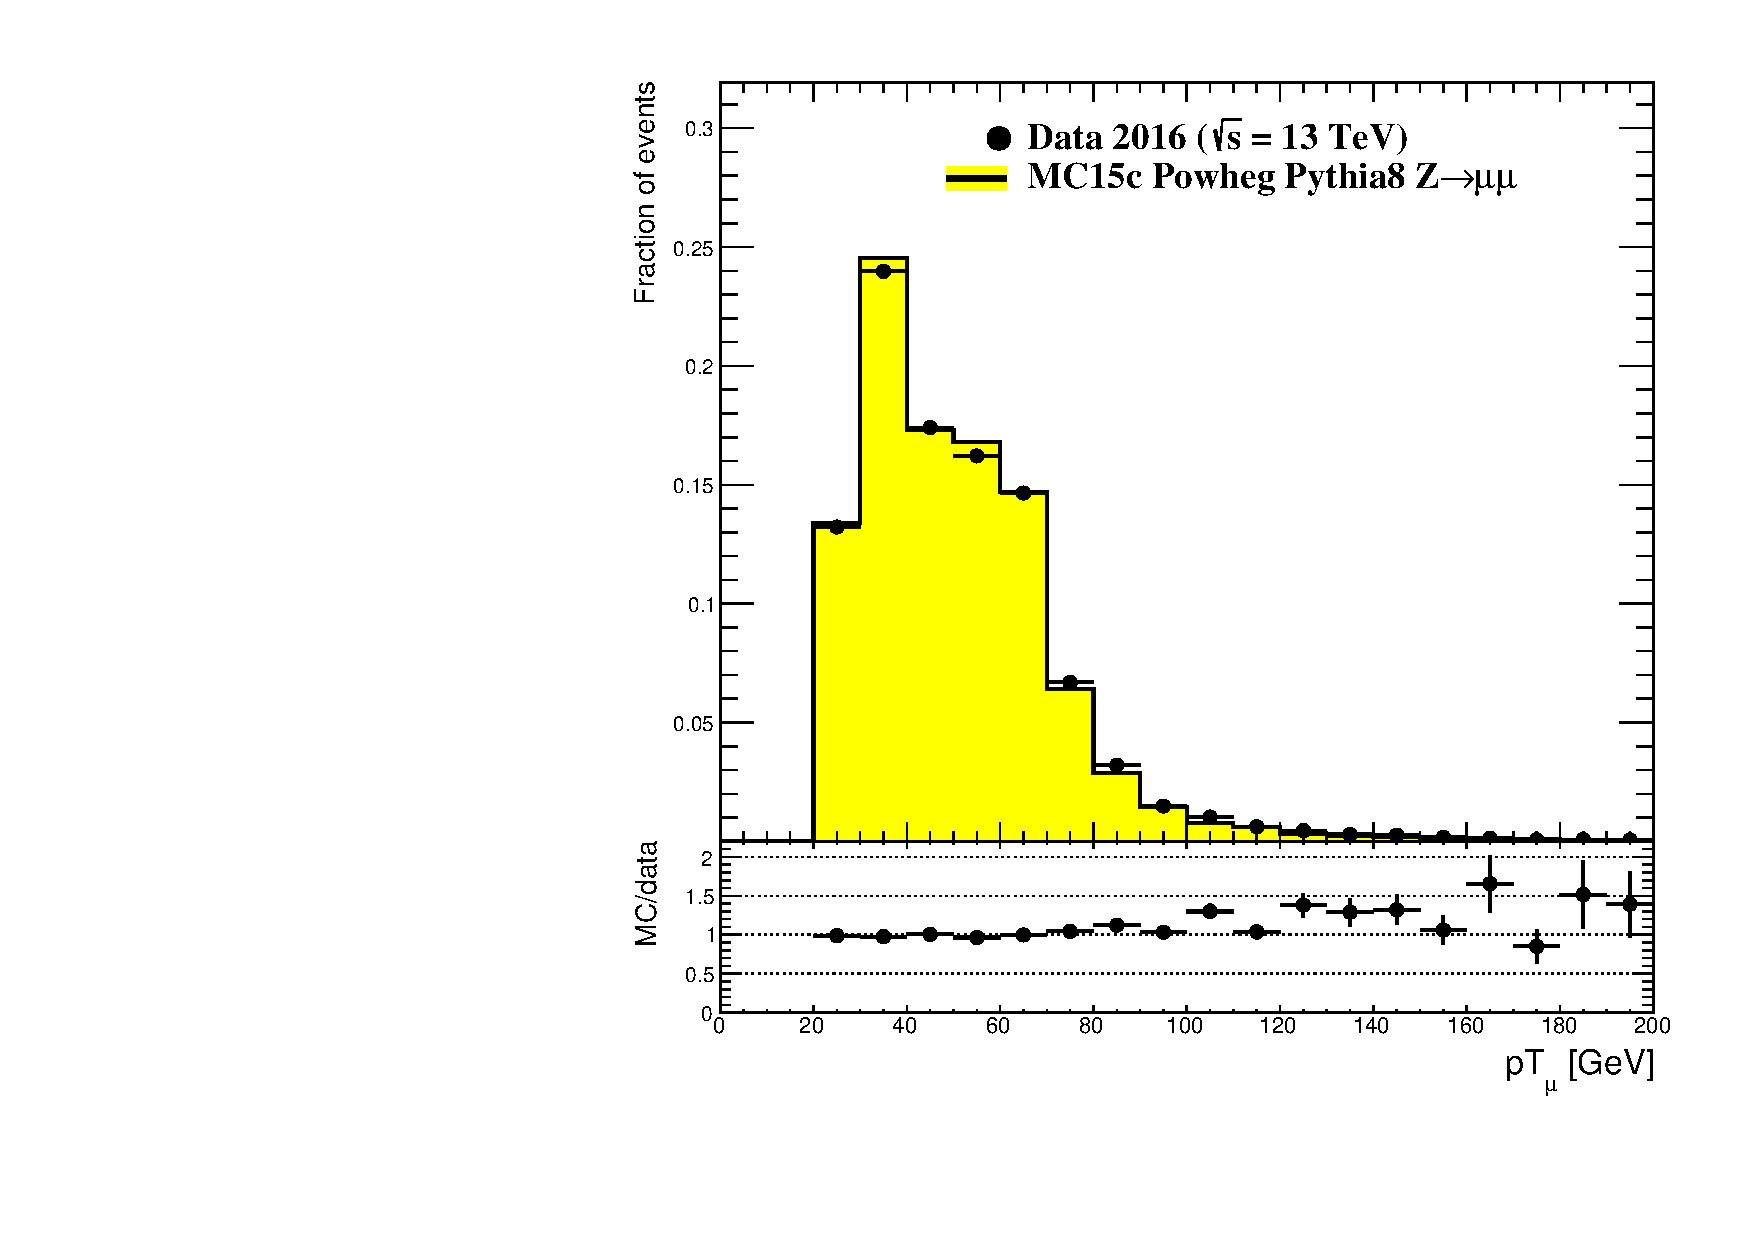
\includegraphics[width=0.53\figwidth]{muon_ptratio}
\caption[Transversal momentum of the muons]{$pT_{\mu}$}
\label{fig:muonpt}
\end{subfigure}
\quad
\begin{subfigure}[b]{0.5\figwidth}
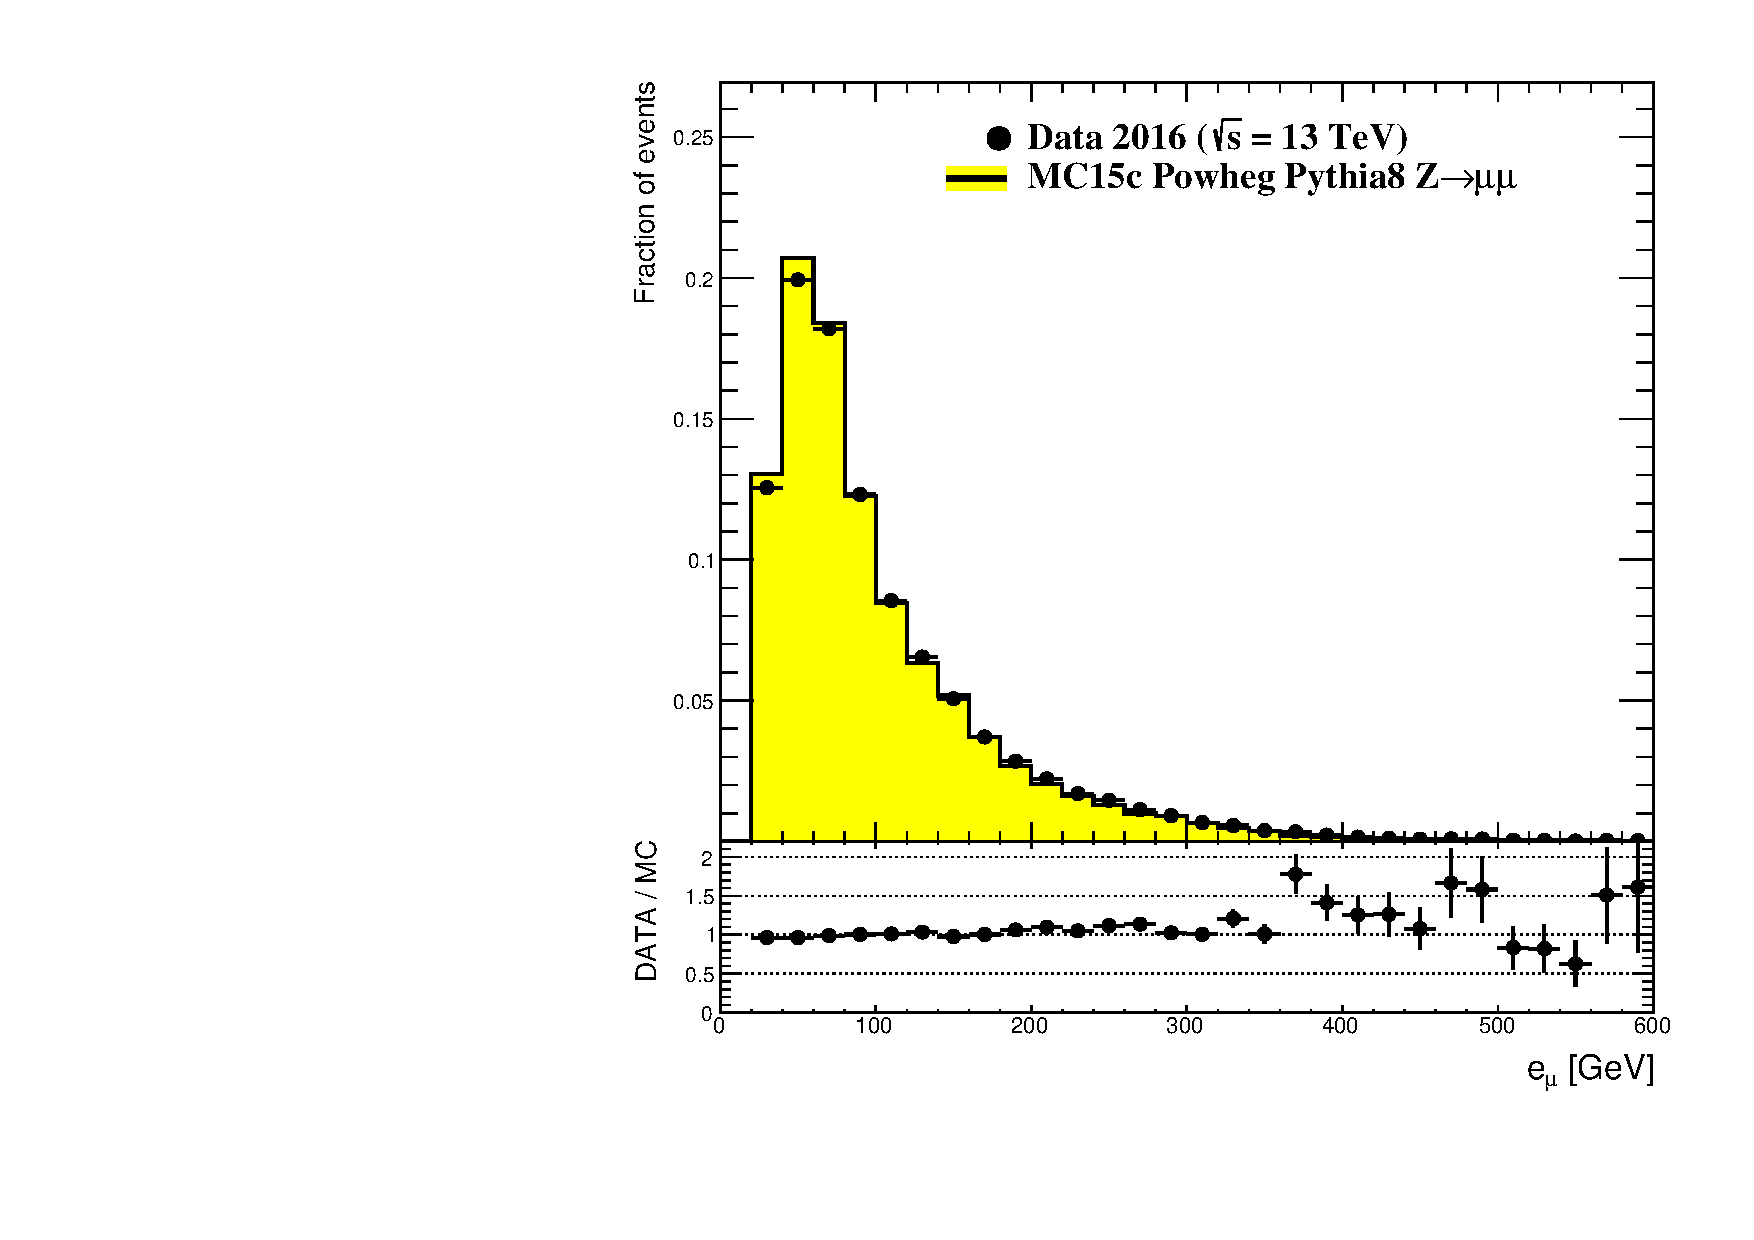
\includegraphics[width=0.53\figwidth]{muon_eratio}
\caption[Energy of the muons]{$e_{\mu}$}
\label{fig:muone}
\end{subfigure}
%\end{figure}


%\begin{figure}[h]
%\centering
\begin{subfigure}[b]{0.5\figwidth}
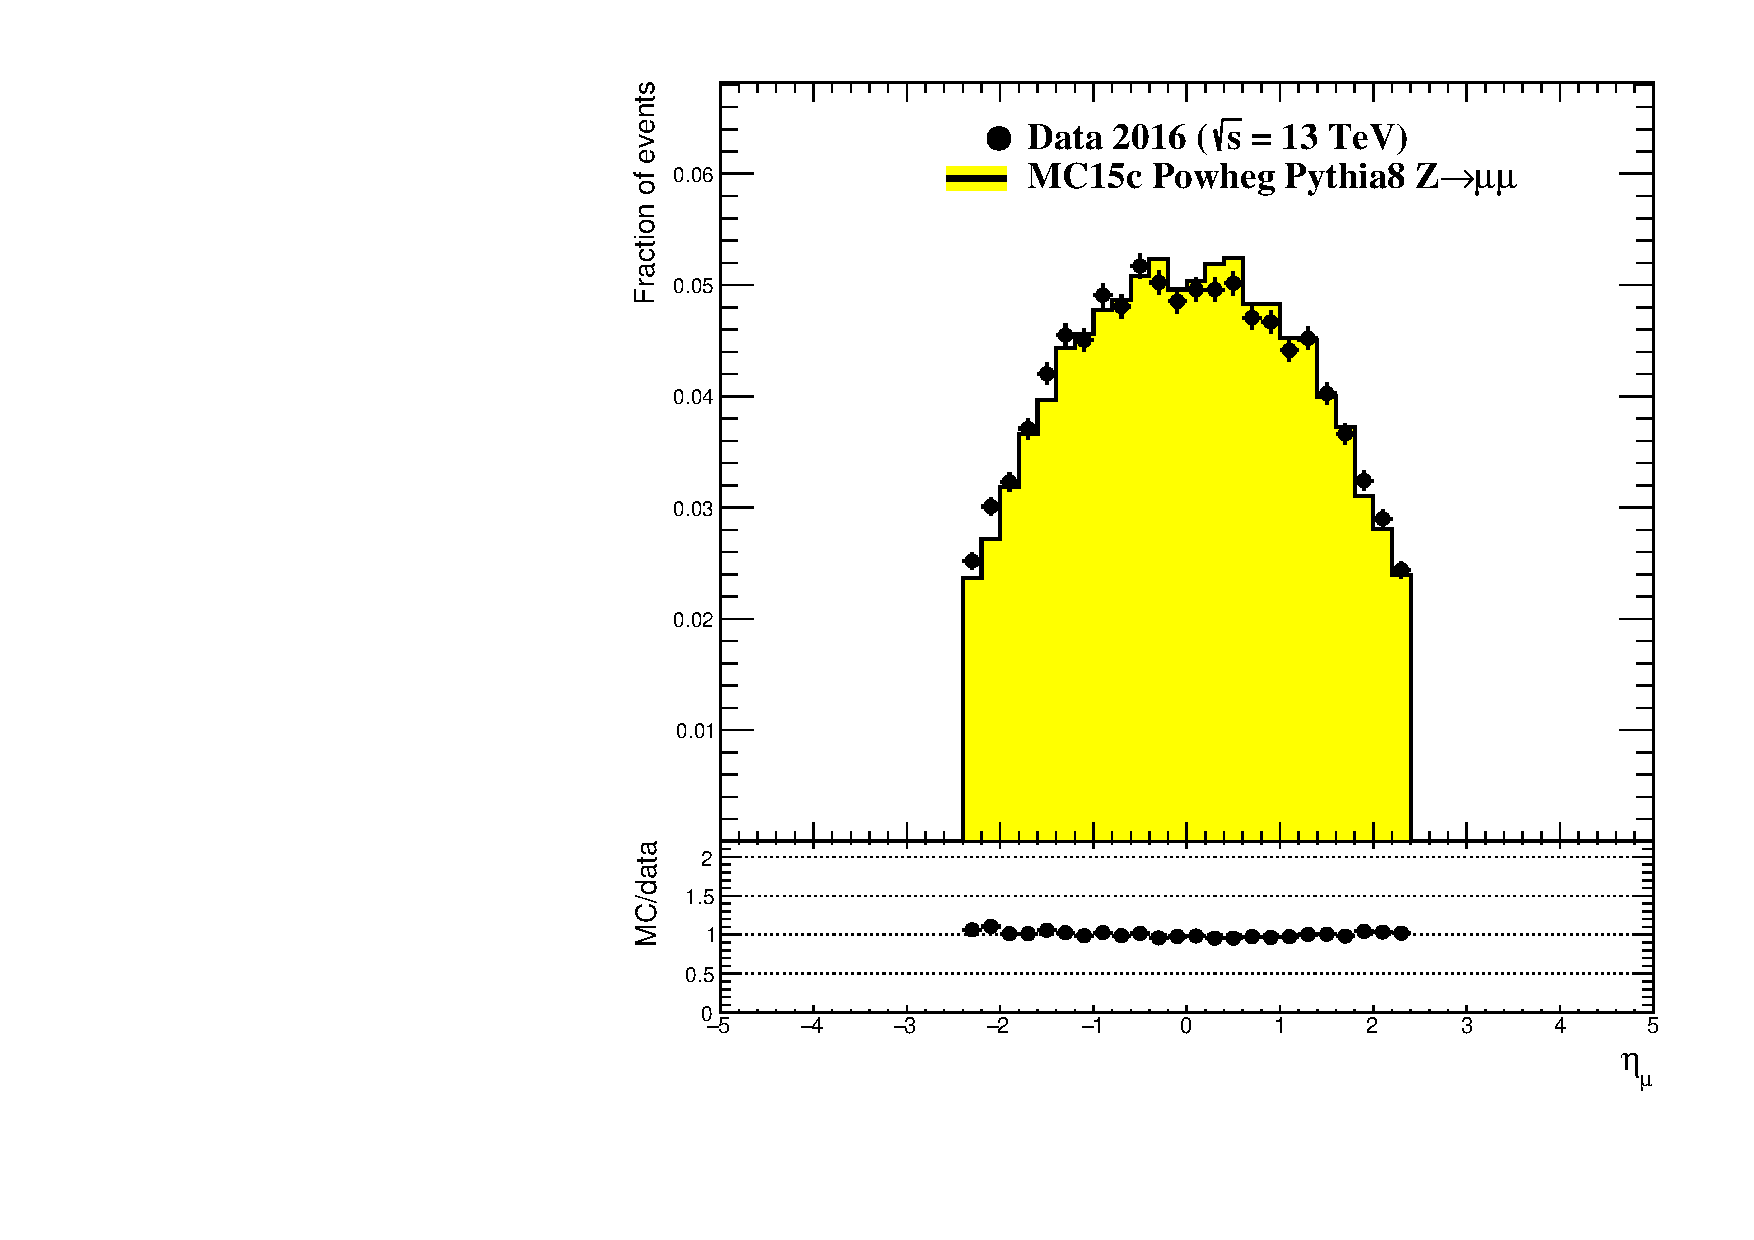
\includegraphics[width=0.53\figwidth]{muon_etaratio}
\caption[$\eta$ of the muons]{$\eta_{\mu}$}
\label{fig:muoneta}
\end{subfigure}
\quad
\begin{subfigure}[b]{0.5\figwidth}
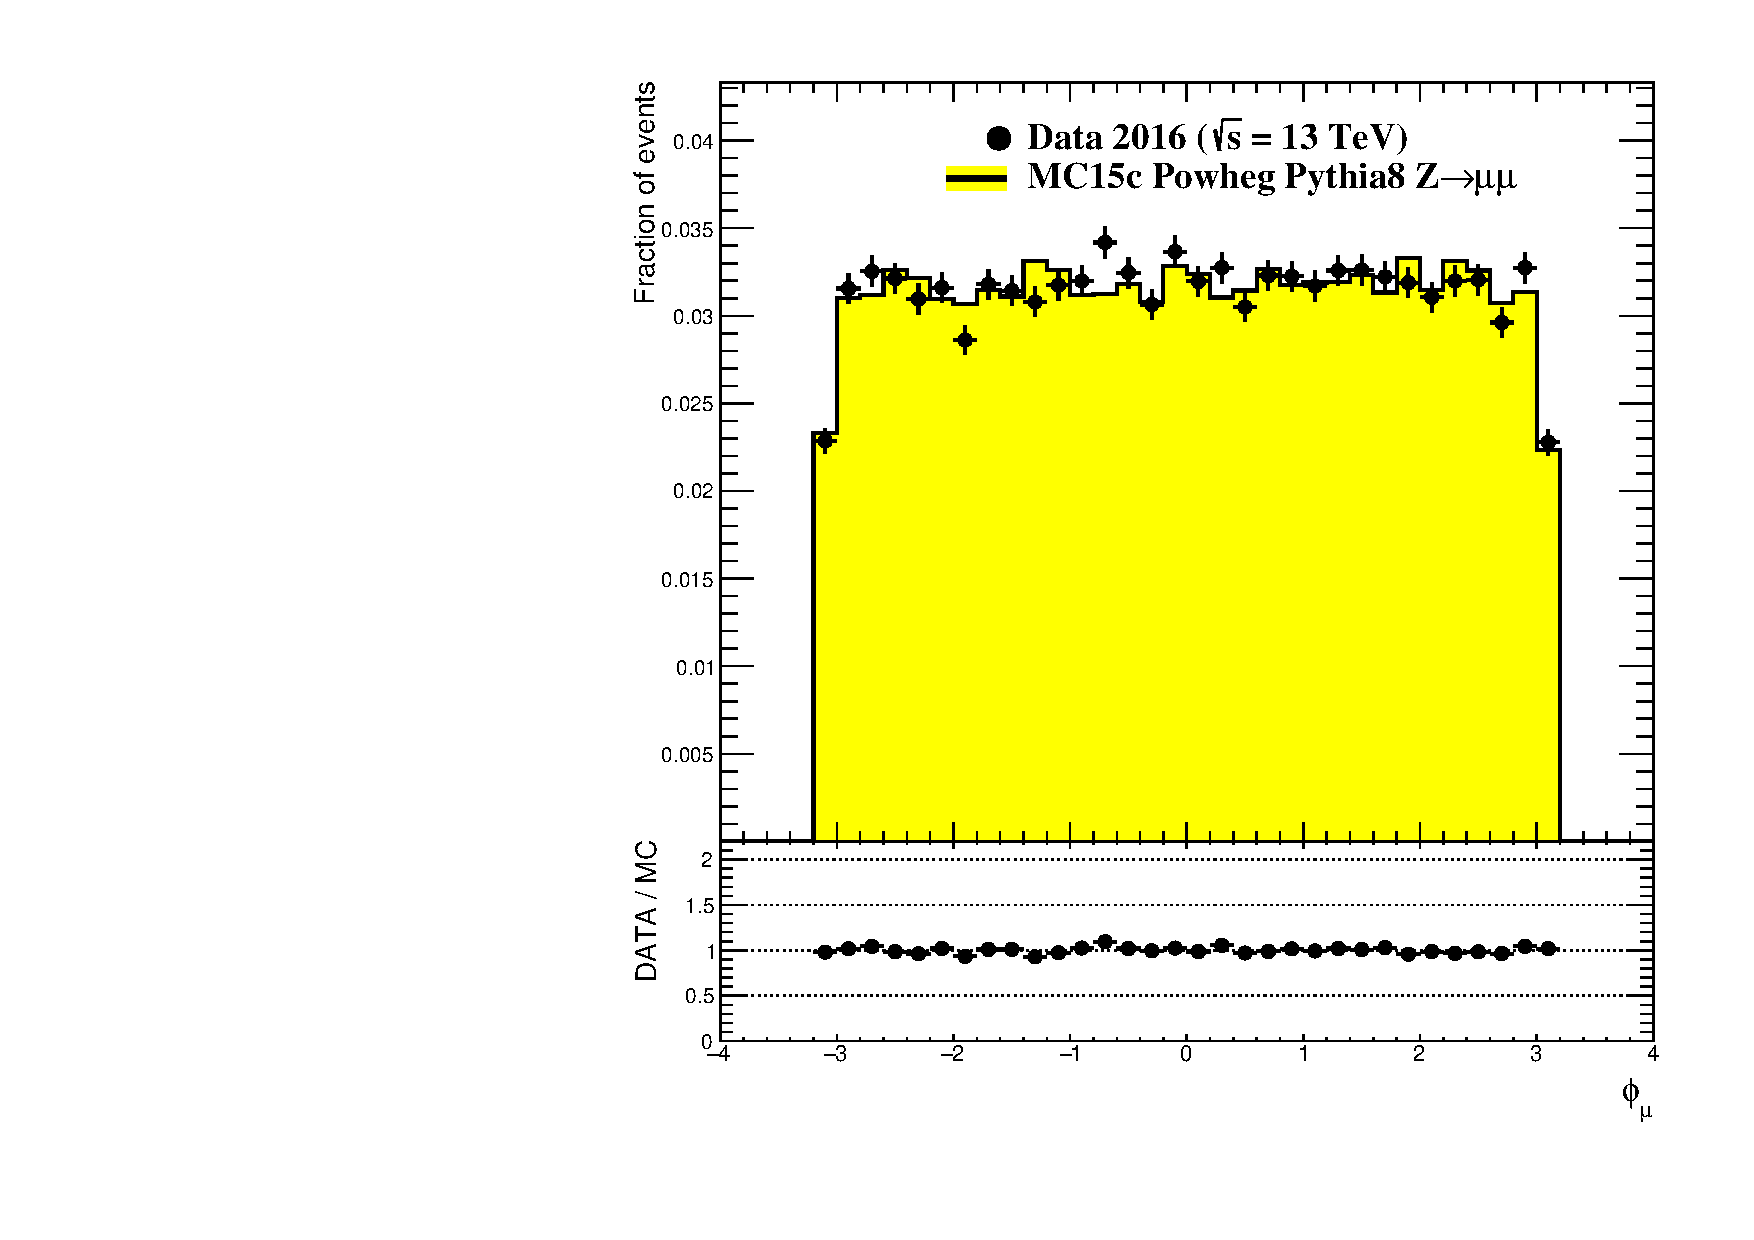
\includegraphics[width=0.53\figwidth]{muon_phiratio}
\caption[$\phi$ of the muons]{$\phi_{\mu}$}
\label{fig:muonphi}
\end{subfigure}
\caption{Properties of the two muons. The histograms are normalized. The distributions shown are: (a) the transversal momentum of the muons; (b) the muons' energy; (c) the muons' $\eta$ and (d) the muons' $\phi$}
\label{fig:muons}
\end{figure}



\section{Reconstruction of the Z-Boson}

The $Z$-boson is reconstructed from the two muons in the selected event.
It is required to be in an mass range of \SI{90+-10}{\GeV} and to have a transversal momentum greater than \SI{30}{\GeV}.

Figure \ref{fig:z} shows the properties of the reconstructed $Z$ boson in data-MC comparison. The agreement of data and Monte Carlo for the $Z$ is in general very good. The momentum resolution worsens slightly with $pT$ exceeding $\SI{80}{\GeV}$ but keeps a reasonable agreement. The mass of the $Z$ boson fluctuates in a range of about \SI{5}{\GeV} around the expected value of \SI{91.19}{\GeV} and has a good agreement with the MC.
The agreement of the pseudo-rapidity as well as for the planar angle is also very good.


\begin{figure}[h]
\centering
\begin{subfigure}[b]{0.5\figwidth}
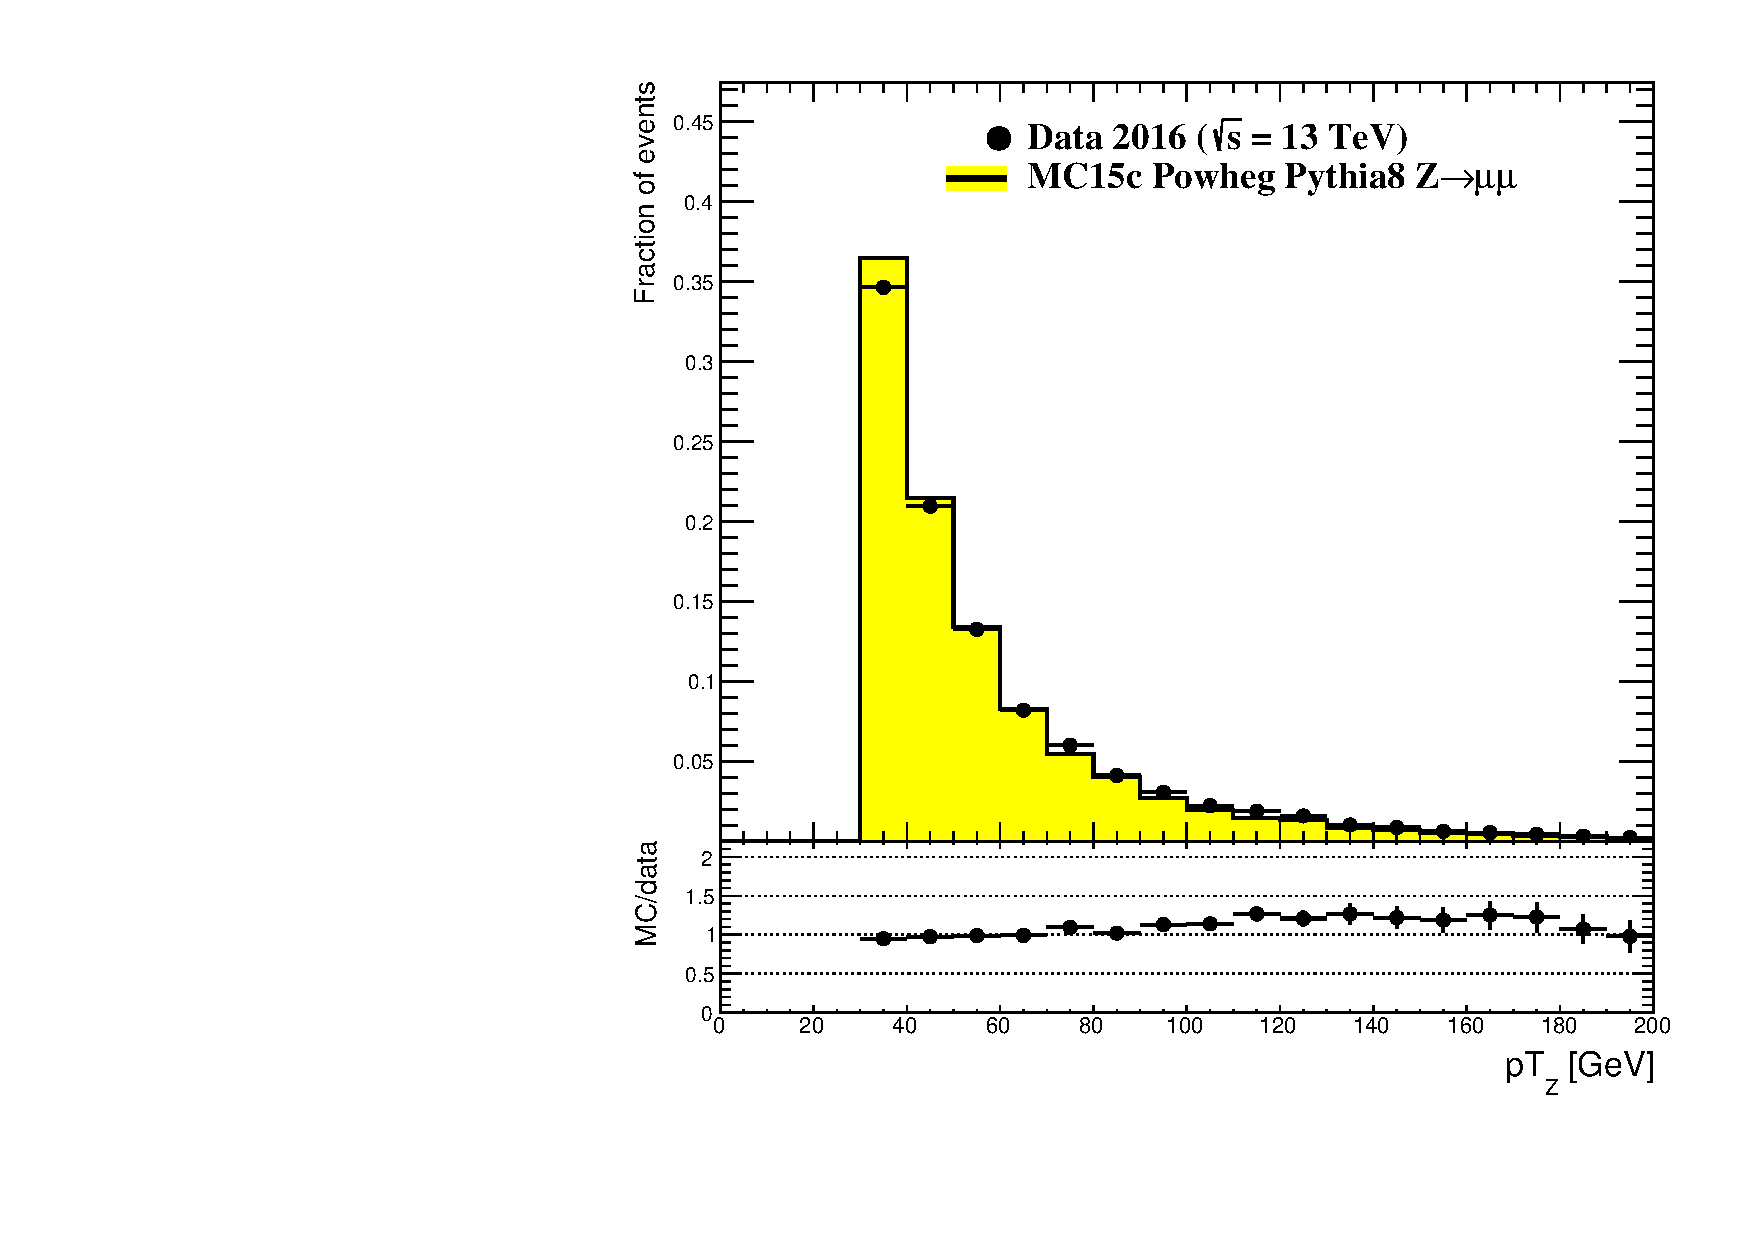
\includegraphics[width=0.53\figwidth]{Z_ptratio}
\caption[Transversal momentum of the reconstructed Z]{$pT_Z$}
\label{fig:zpt}
\end{subfigure}
\quad
\begin{subfigure}[b]{0.5\figwidth}
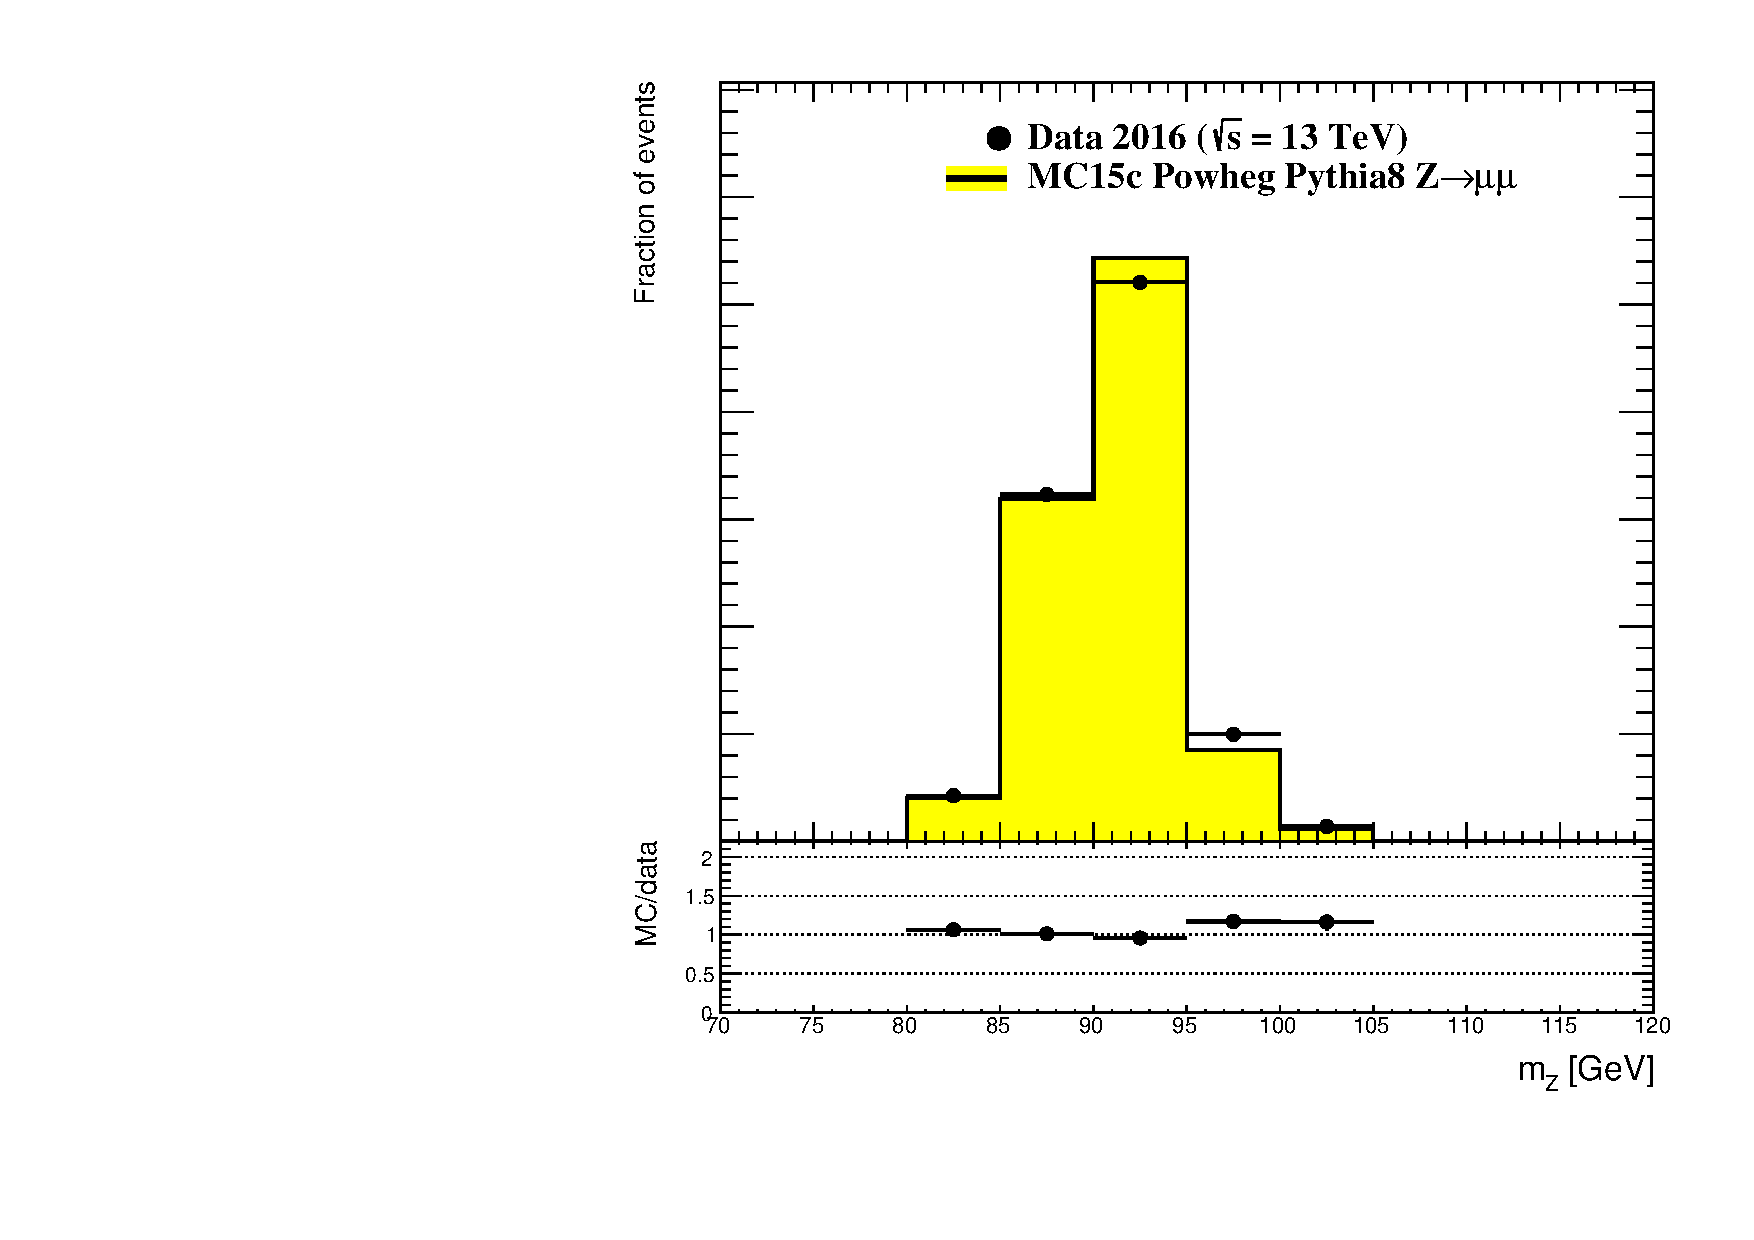
\includegraphics[width=0.53\figwidth]{Z_mratio}
\caption[mass of the reconstructed $Z$]{$m_Z$}
\label{fig:zm}
\end{subfigure}
%\end{figure}


%\begin{figure}[h]
%\centering
\begin{subfigure}[b]{0.5\figwidth}
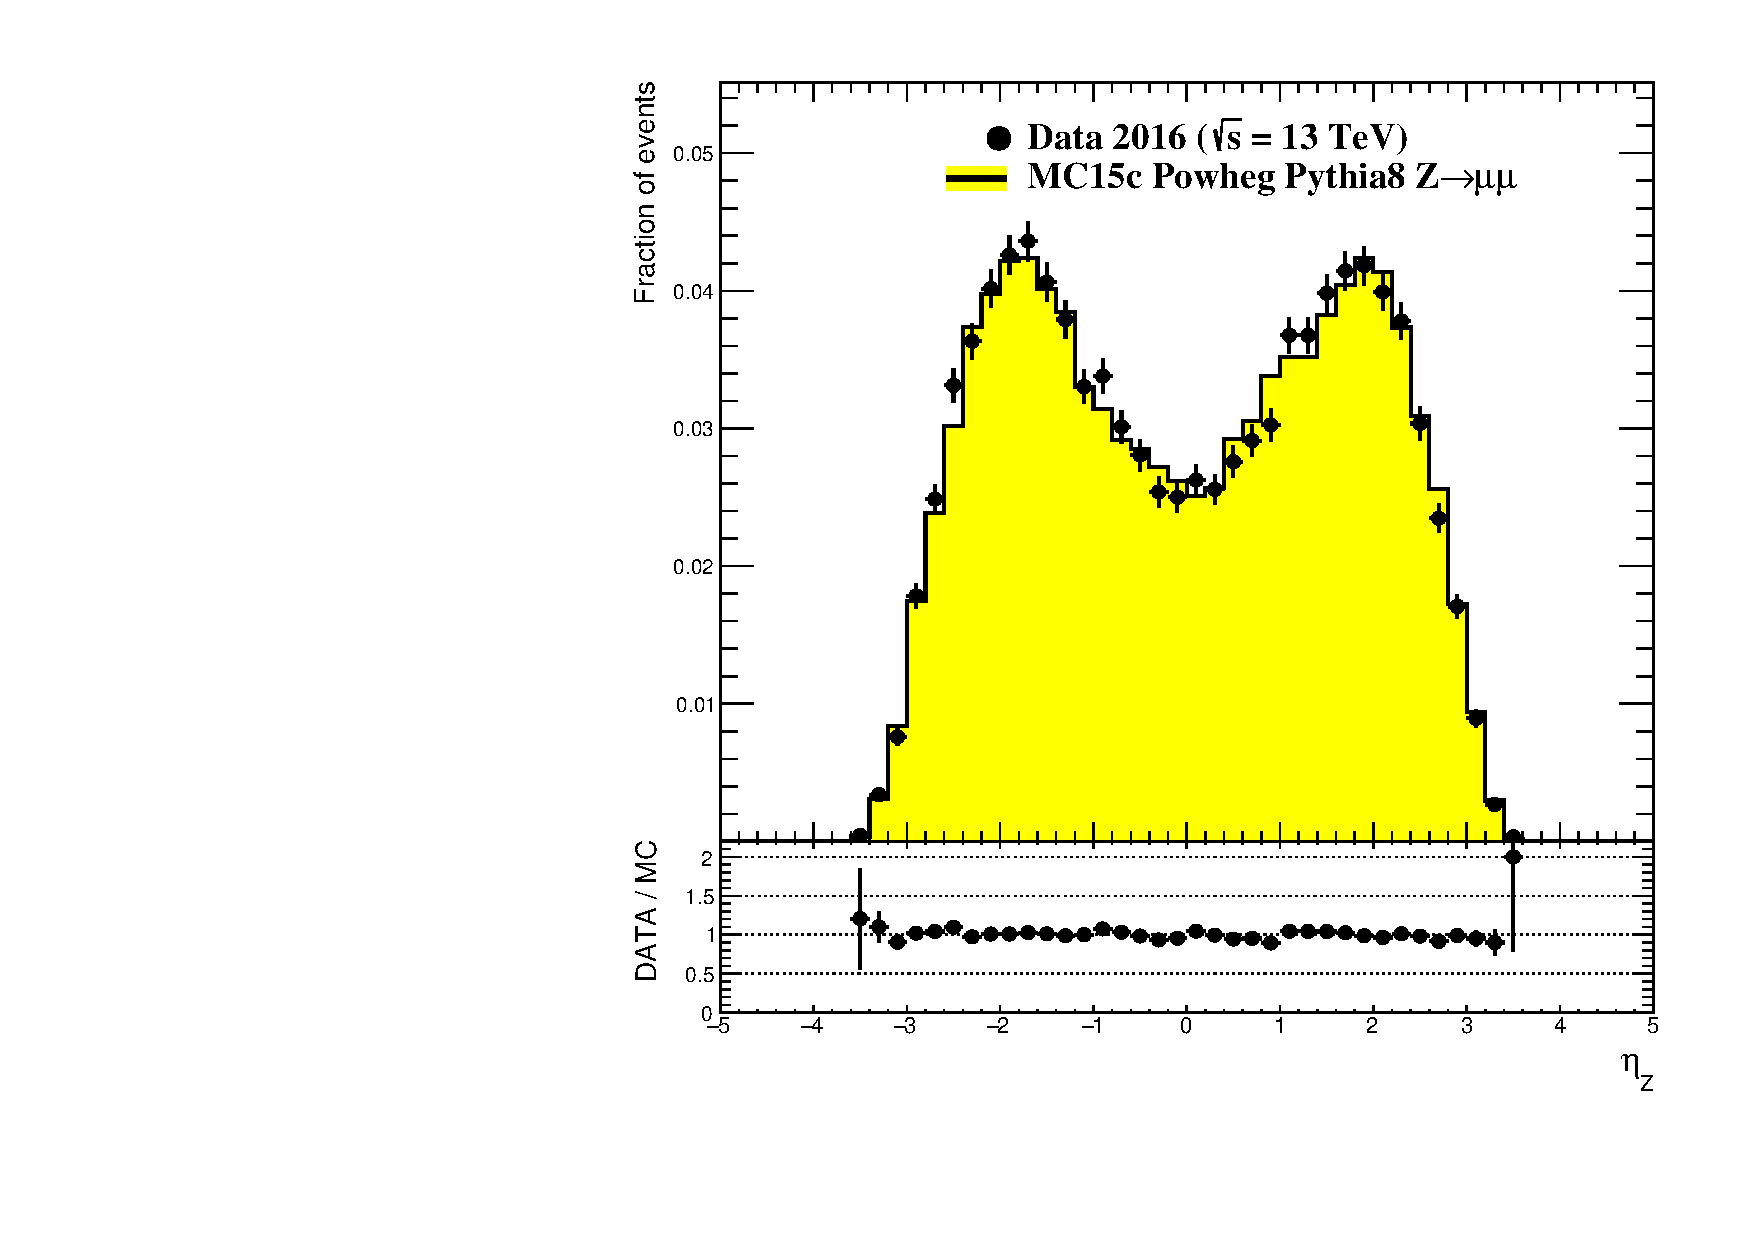
\includegraphics[width=0.53\figwidth]{Z_etaratio}
\caption[$\eta$ of the reconstructed $Z$]{$\eta_Z$}
\label{fig:zeta}
\end{subfigure}
\quad
\begin{subfigure}[b]{0.5\figwidth}
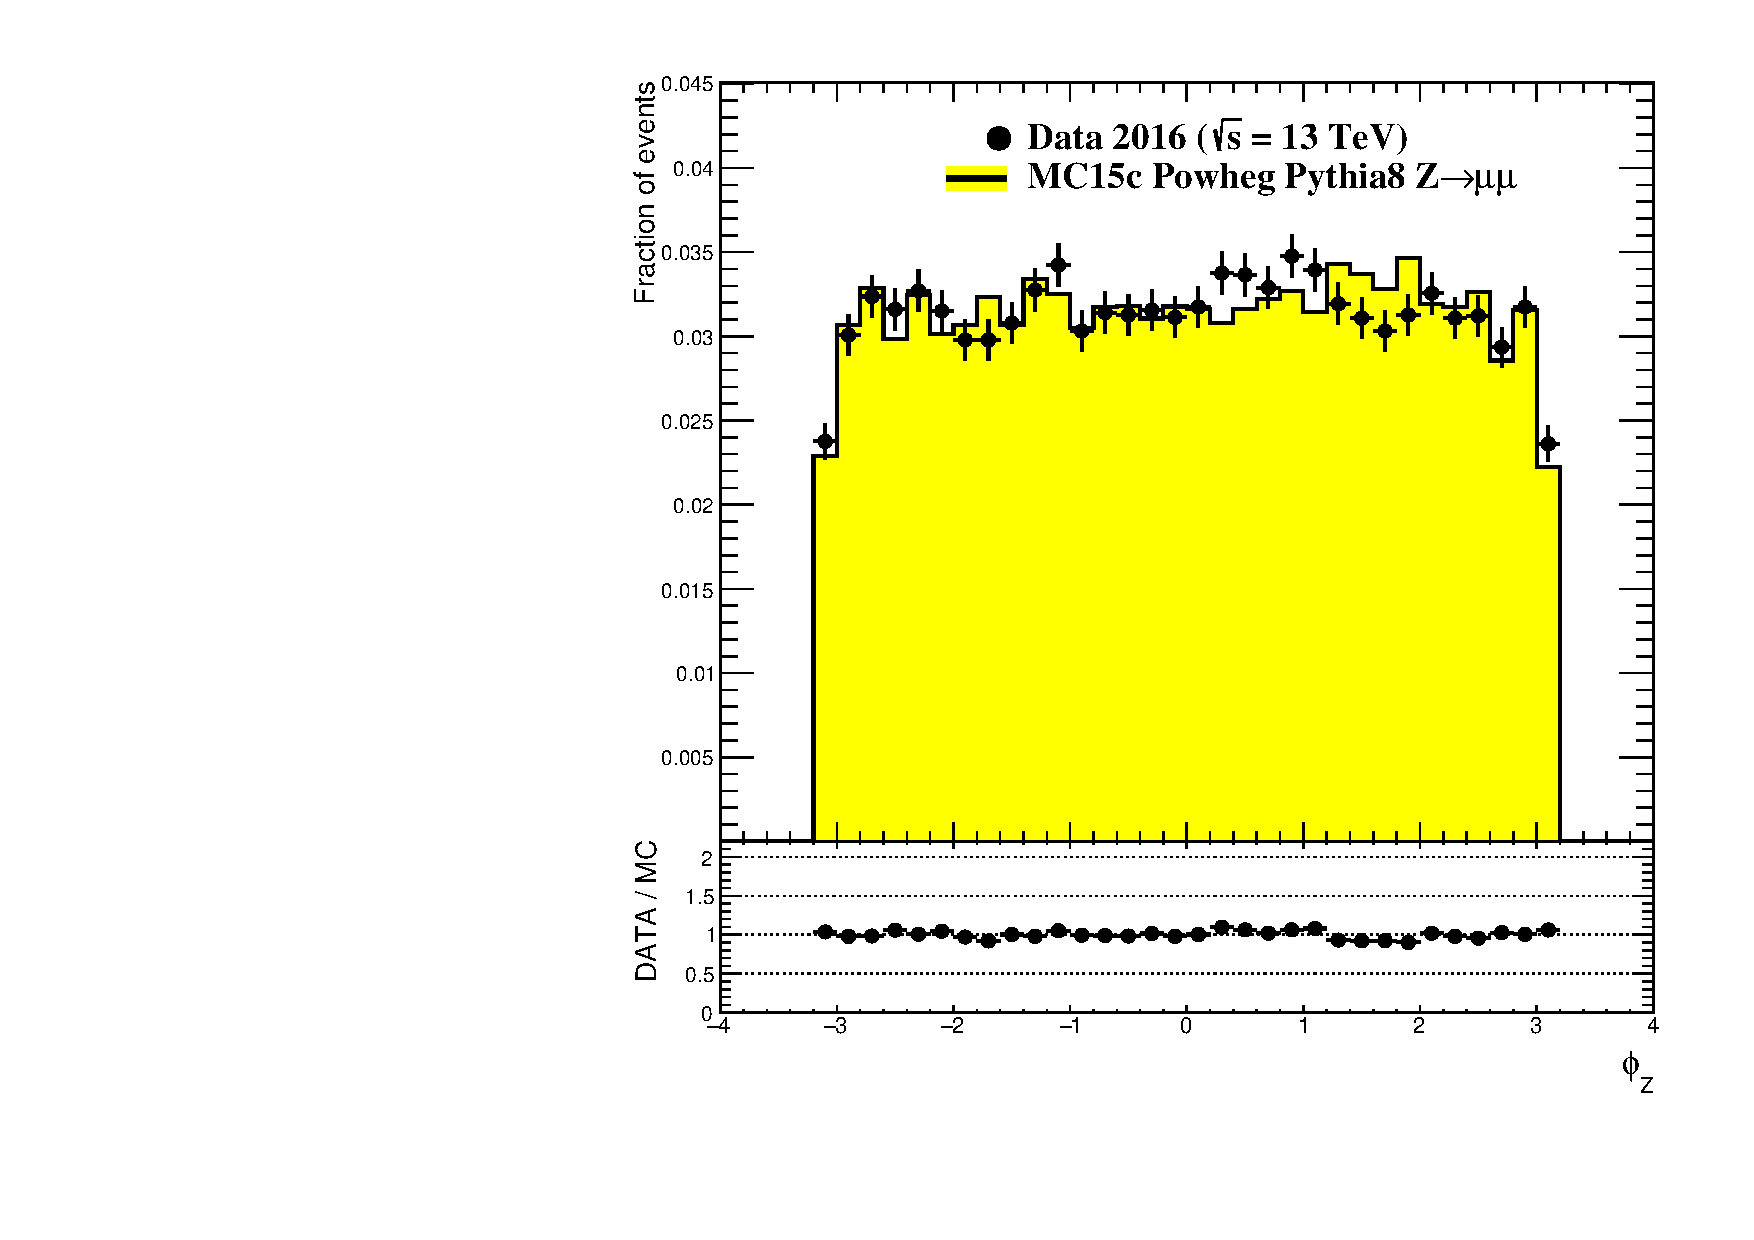
\includegraphics[width=0.53\figwidth]{Z_phiratio}
\caption[$\phi$ of the reconstructed $Z$]{$\phi_Z$}
\label{fig:zphi}
\end{subfigure}
\caption{Properties of the reconstructed Z-Boson. MC and data are normalized to the total number of reconstructed Z bosons. The distributions show (a) the transversal momentum; (b) the mass; (c) the pseudo-rapidity and (d) the $\phi$ of the $Z$.}
\label{fig:z}
\end{figure}

\section{Kinematic variables of the recoiling jets}

To select the jets recoiling to the $Z$ bosons a further selection is applied to a given $Z \rightarrow \mu \mu$ event. The criteria are as follows:

\begin{itemize}
\item The jet is required to have a transverse momentum greater than \SI{20}{\GeV}.
\item The jet is required to be recoiling to the reconstructed Z. The criteria is $|\phi_{jet}-\phi_Z|<(\pi - \num0.4)$.
\item Due to the limited region of the tracking detector the pseudo-rapidity of the jet is restricted to $|\eta|<2.5$.
\end{itemize}

The kinematic properties of the recoiling jet are shown in figure \ref{fig:reoilingjet}. The agreement for $pT$ and energy are rather bad for the jets especially in high energy regions compared to the agreement seen for muons and the reconstructed Z and even in low $pT$ and energy regions there is a clearly noticeable difference between the two distributions. But in general the shapes for both distributions are well comparable and there is no complete disagreement. The results are close enough to let a good agreement to be expected affter further improvements in calibration and scaling. 
The angular agreement looks better except for $|\eta|>2.5$ which is outside the tracker region and could be excluded for Particle Flow performance analysis.

Figure \ref{fig:generalproperties} shows the comparison of data and Monte Carlo for some further jet variables.

%The first distribution shows the number of vertices per %event. The agreement between data and MC is rather bad. %The center of the MC-distribution is displaced to the %left with respect to the data distribution. This %suggests that the MC needs further weighting to match %the data better. Given that the completion of the %weighting is still in process one can hope that a proper %weighting of the vertices might also improve other %distributions. Nevertheless the distributions for data %and MC are comparable and show similar shapes.

The first distribution \ref{fig:chfrac} shows the fraction of jet-$pT$ carried by reconstructed tracks. The agreement is decent. The first bin here is not an overflow bin but refers to neutral objects. There are going to be further studies needed to find the origin of this immense fraction of neutral objects.

The second distribution \ref{fig:trackcount} shows the number of tracks in a jet. The agreement worsens for a high track multiplicity. This might be due to insufficient statistics. Furthermore there might be wrong tracks reconstructed in data because the data multiplicity generally is higher that in MC.

The last distribution \ref{fig:trackwidth} shows the track width. The agreement is reasonable although the fluctuations can hopefully be mediated by further scaling.



\begin{figure}[h]
\centering
\begin{subfigure}[b]{0.5\figwidth}
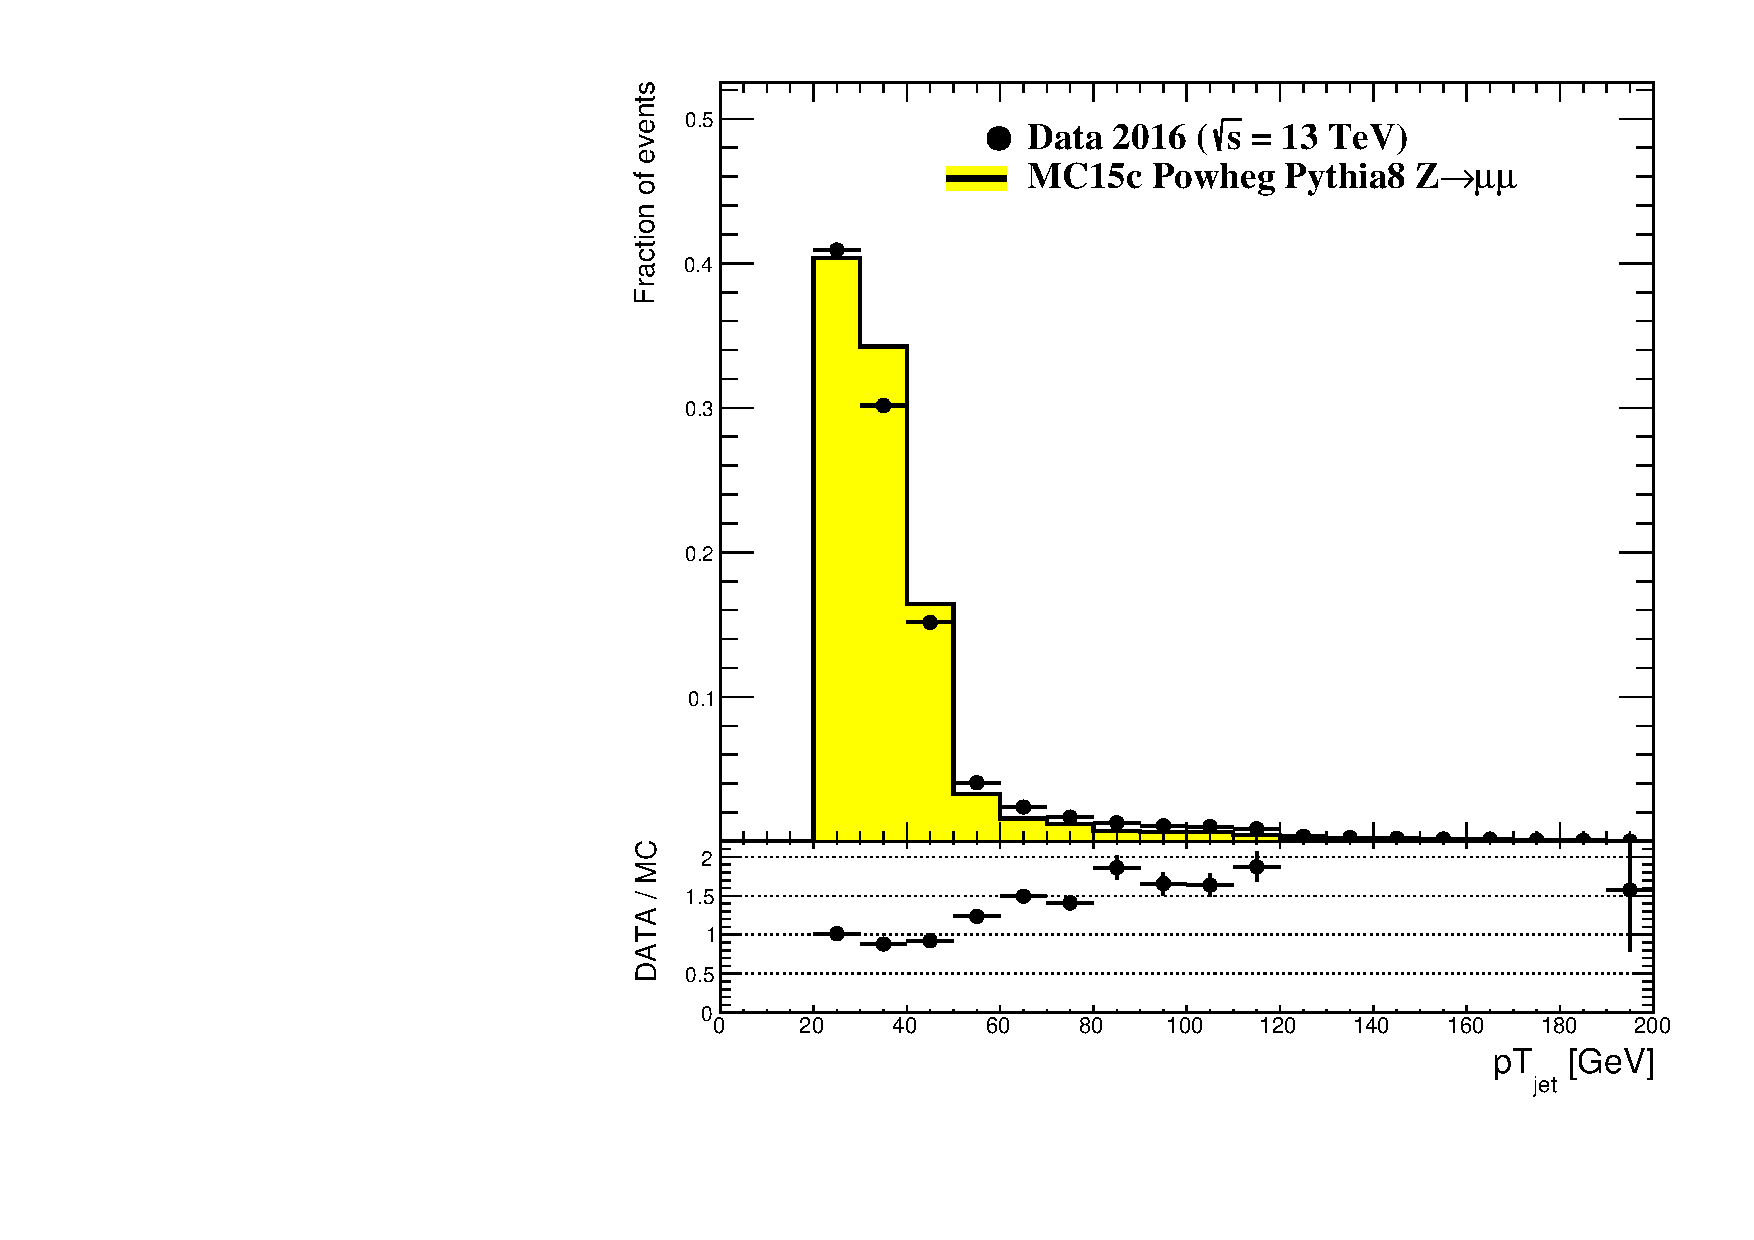
\includegraphics[width=0.53\figwidth]{jet_ptratio}
\caption[Transversal momentum of the recoiling jet]{$pT_{jet}$}
\label{fig:jetpt}
\end{subfigure}
\quad
\begin{subfigure}[b]{0.5\figwidth}
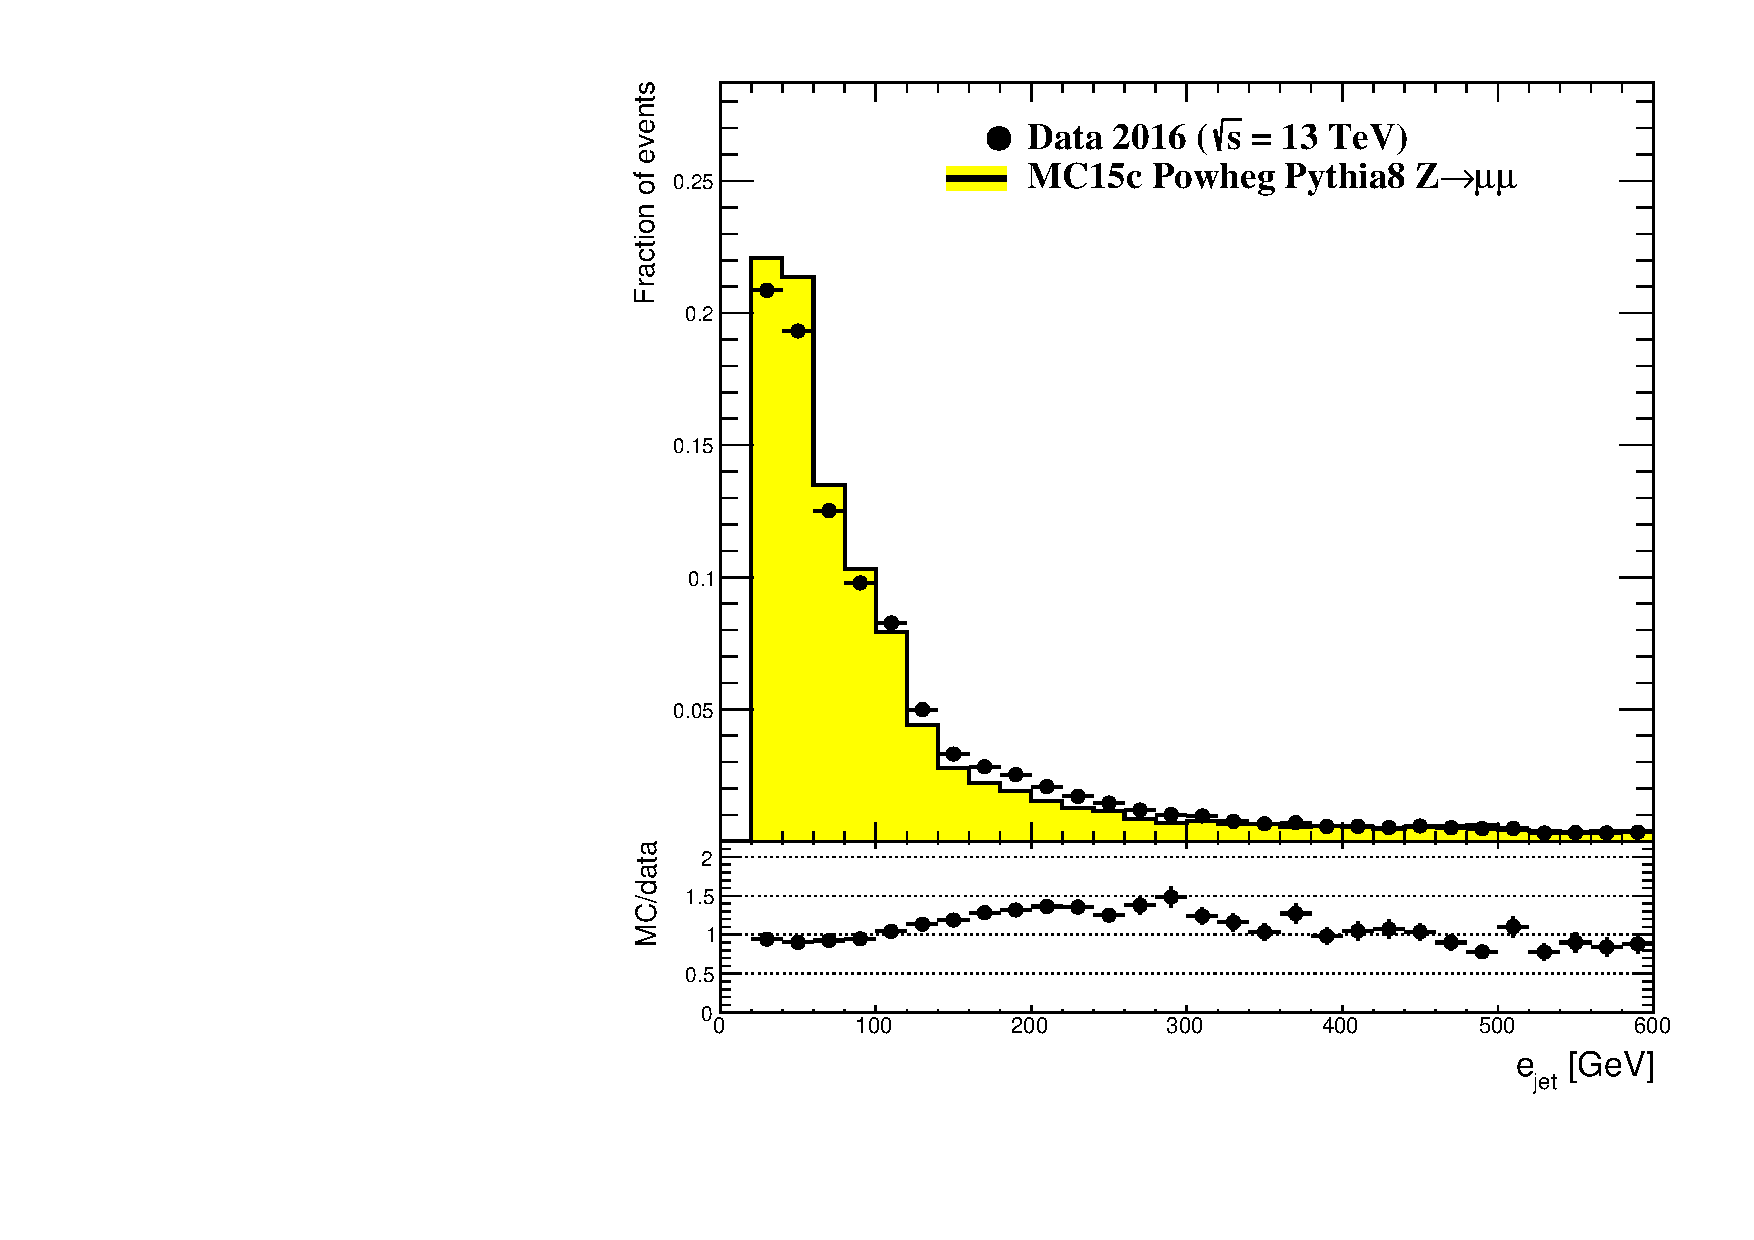
\includegraphics[width=0.53\figwidth]{jet_eratio}
\caption[Energy of the recoiling jet]{$e_{jet}$}
\label{fig:jete}
\end{subfigure}
%\end{figure}


%\begin{figure}[h]
%\centering
\begin{subfigure}[b]{0.5\figwidth}
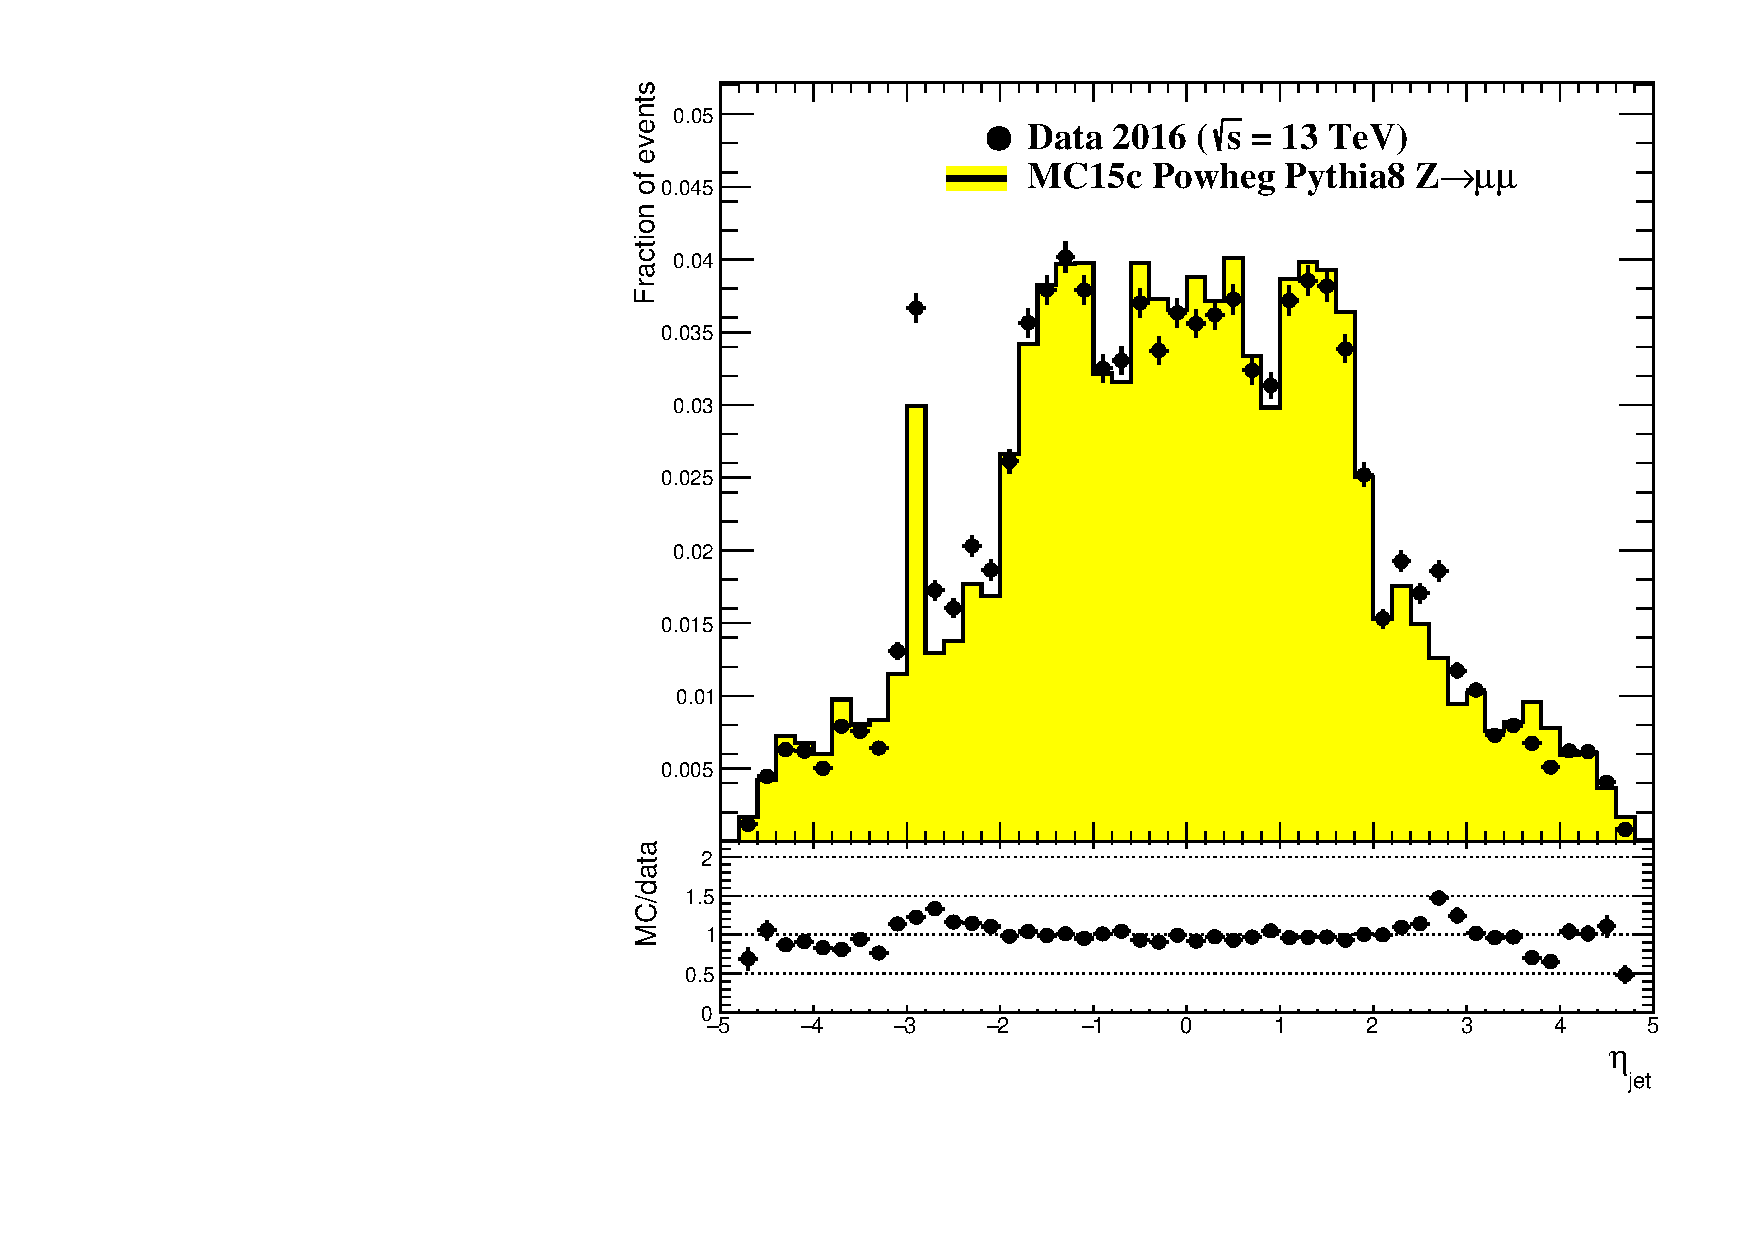
\includegraphics[width=0.53\figwidth]{jet_etaratio}
\caption[$\eta$ of the recoiling jet]{$\eta_{jet}$}
\label{fig:jeteta}
\end{subfigure}
\quad
\begin{subfigure}[b]{0.5\figwidth}
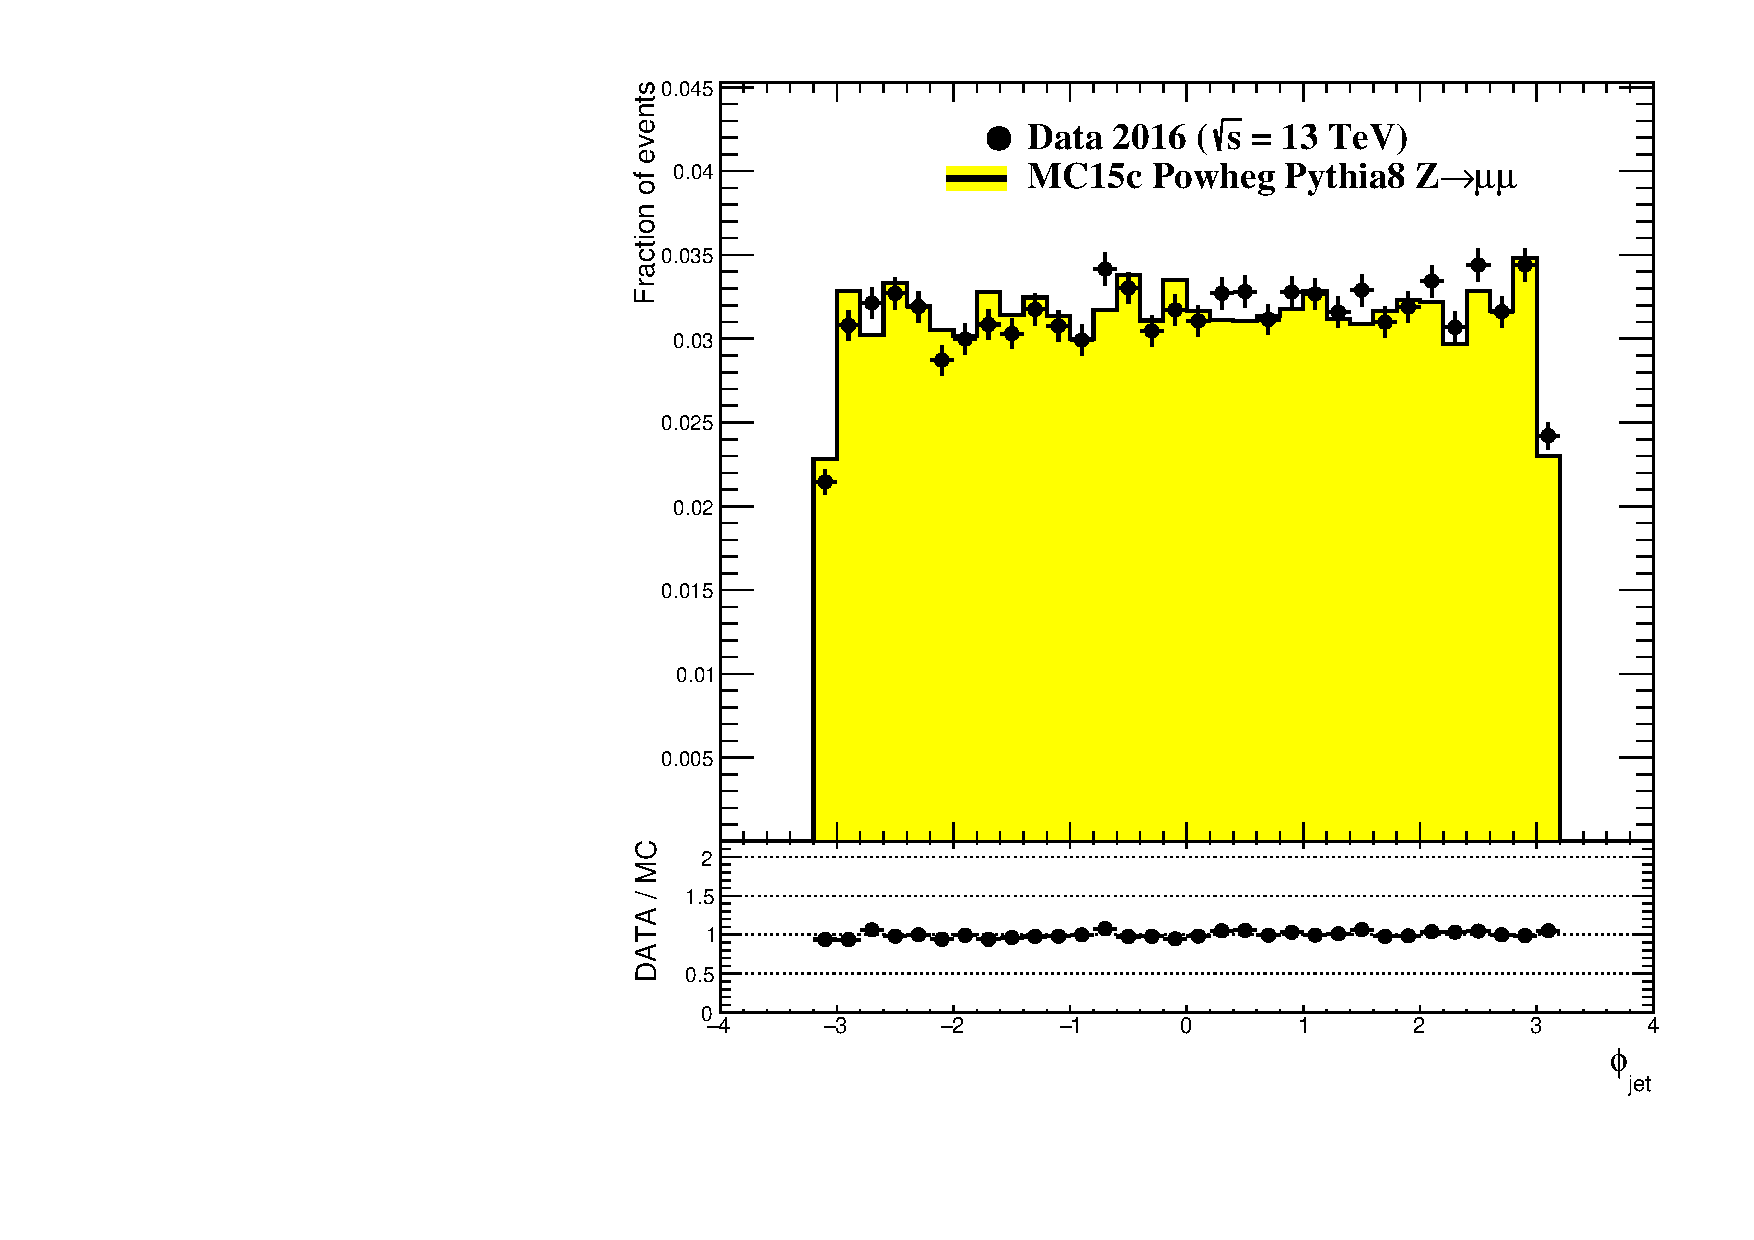
\includegraphics[width=0.53\figwidth]{jet_phiratio}
\caption[$\phi$ of the recoiling jet]{$\phi_{jet}$}
\label{fig:jetphi}
\end{subfigure}
\caption{Properties of the recoiling jet. The distributions are normalized to the number of jets. Distributions shown are: (a) the jet's transversal momentum; (b) the jet's energy; (c) the jet's eta and (d) the jet's phi.}
\label{fig:reoilingjet}
\end{figure}




\begin{figure}[h]
\centering
%\begin{subfigure}[b]{0.5\figwidth}
%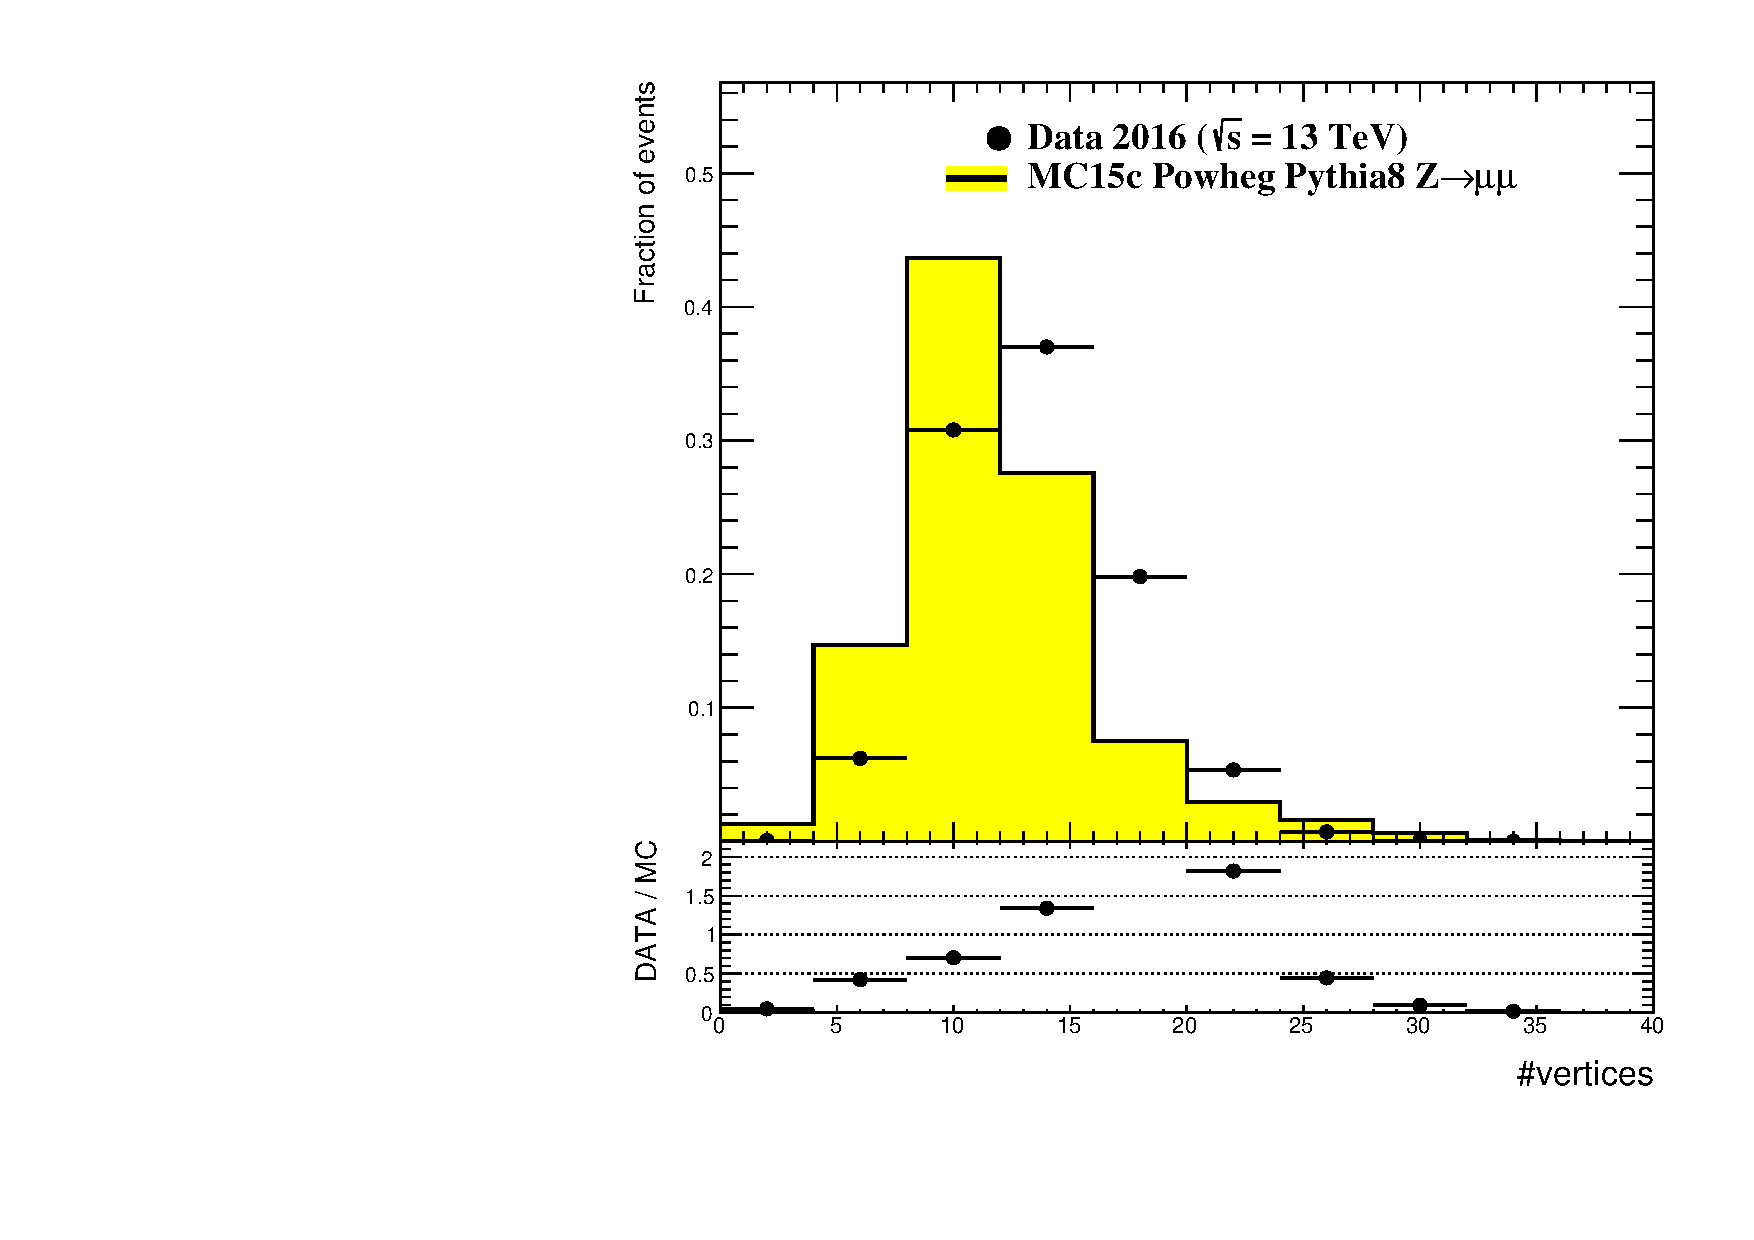
\includegraphics[width=0.53\figwidth]{verticesratio}
%\caption[Number of vertices]{Number of vertices}
%\label{fig:vertices}
%\end{subfigure}
%\quad
\begin{subfigure}[b]{0.5\figwidth}
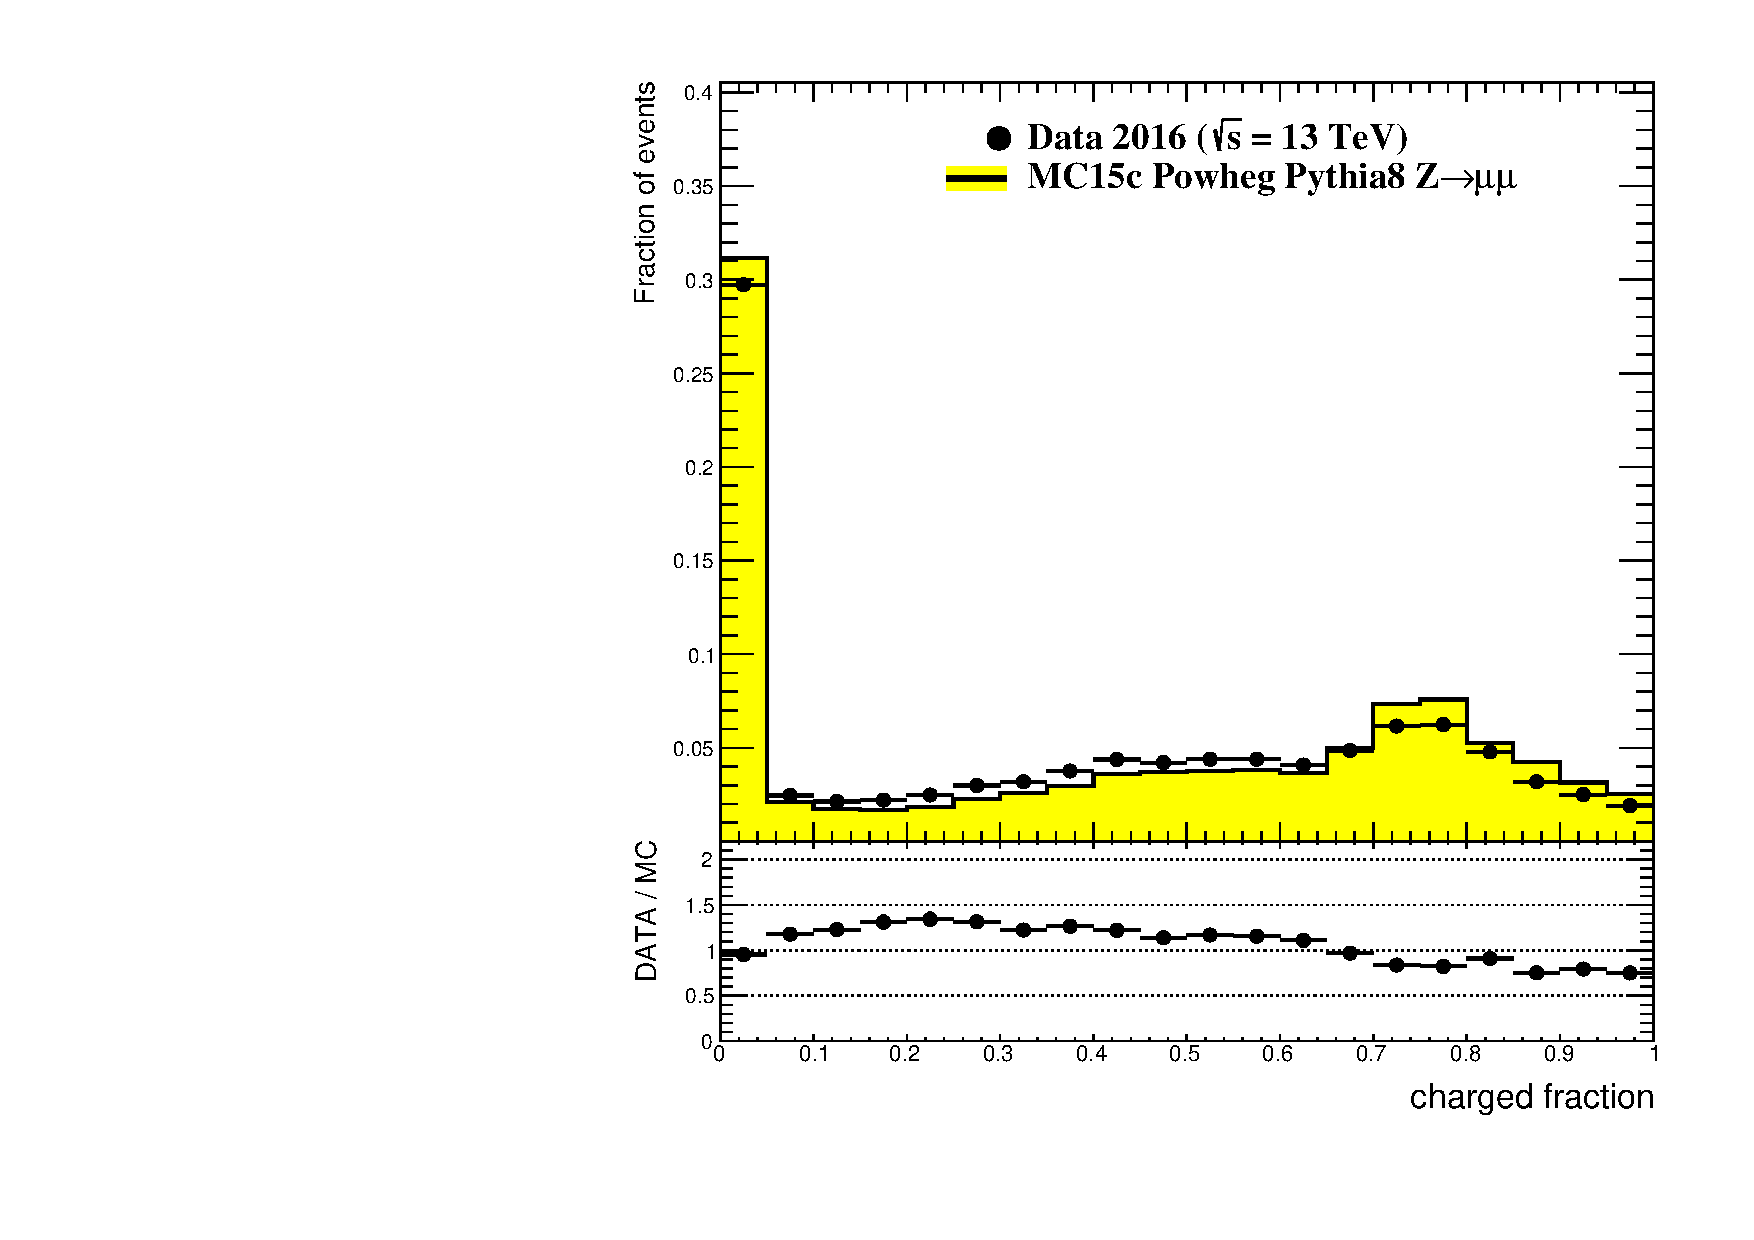
\includegraphics[width=0.53\figwidth]{chfracratio}
\caption[Charged fraction]{Charged fraction}
\label{fig:chfrac}
\end{subfigure}
%\end{figure}


%\begin{figure}[h]
\centering
\begin{subfigure}[b]{0.5\figwidth}
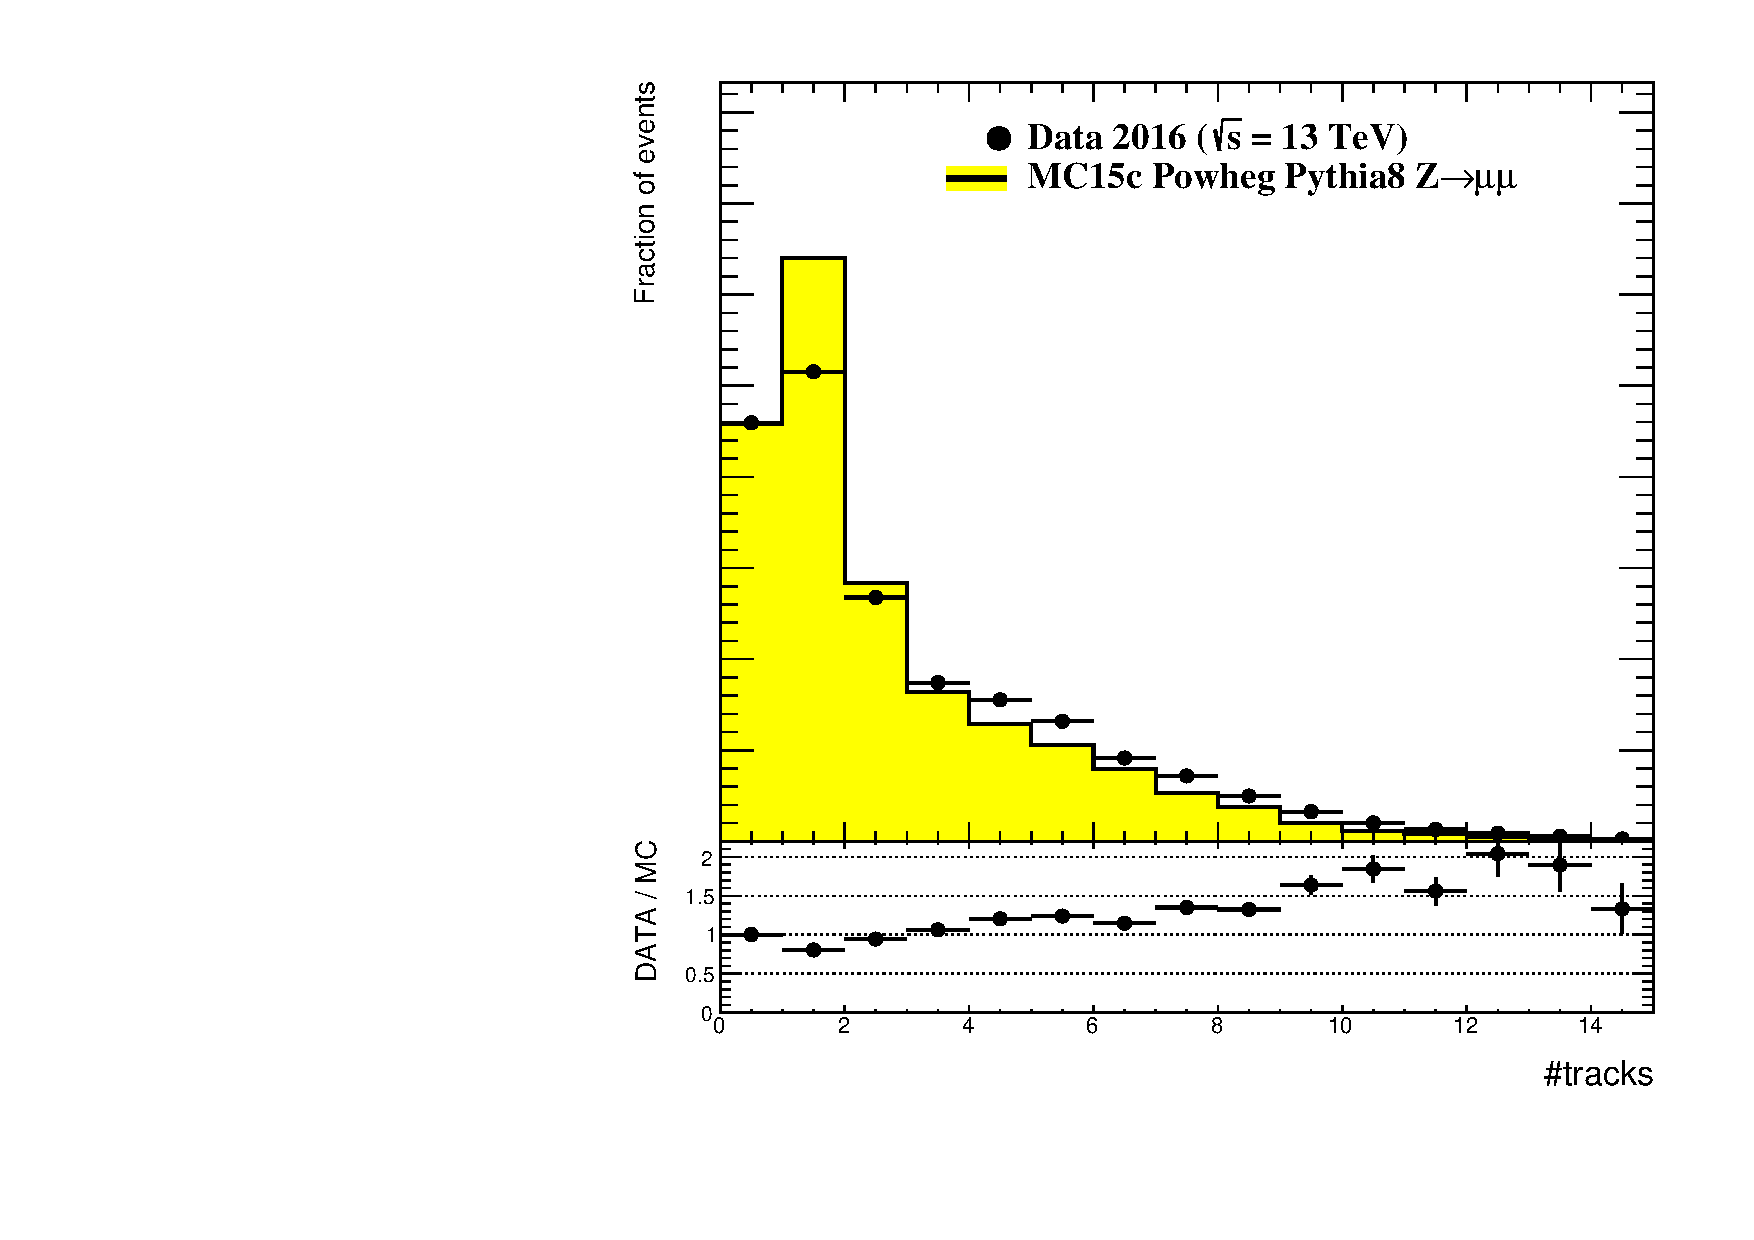
\includegraphics[width=0.53\figwidth]{trackcountratio}
\caption[Track count]{Track count}
\label{fig:trackcount}
\end{subfigure}
\quad
\begin{subfigure}[b]{0.5\figwidth}
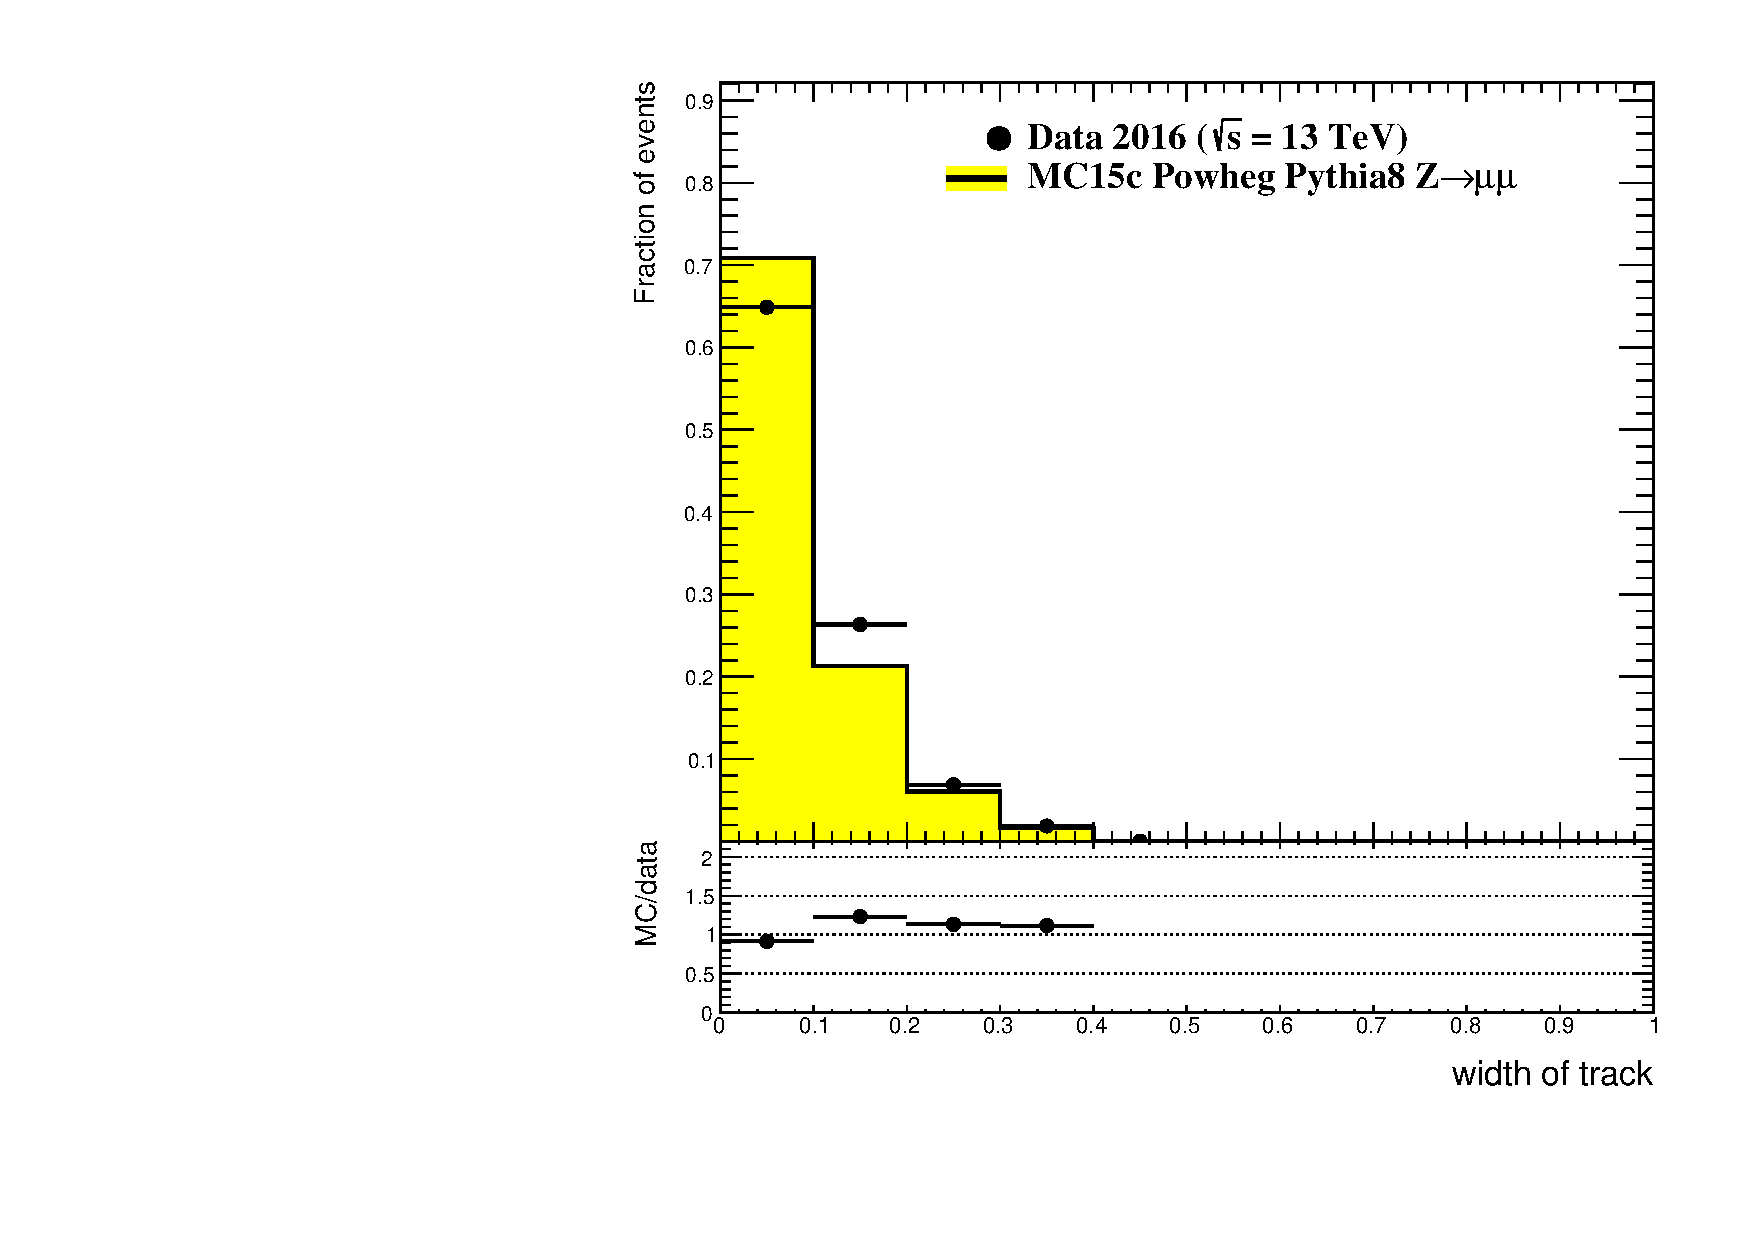
\includegraphics[width=0.53\figwidth]{trackwidthratio}
\caption[trackwidth]{Track width}
\label{fig:trackwidth}
\end{subfigure}
\caption{Further properties of the recoiling jet in data/MC comparison. The distributions are normalized to the sample size. The following distributions are shown: (a) the charged fraction, i.e. the fractional jet $p_T$ carried by reconstructed tracks; (b) the number of tracks in the jet; (c) the track's width.}
\label{fig:generalproperties}
\end{figure}


\section{Conclusion of the performance}

All things considered the data/MC comparison shows that the Particle Flow framework is on a good way. The general shapes of all distributions in our study match well and there are nos gins of major problems.

Right now a full jet calibration as well as jet cleaning for Particle Flow jets is not available. Furthermore the scale factors for all objects and further re-weighting for MC and data have to be applied.
With the improvements expected from these additional tools it is very likely that similar or better results as in Run 1 can be achieved using the Particle Flow algorithm.


\label{results}
